
\chapter{Optimising embedded array programs}
\label{ch:optimising}
\epigraph{Relax. As usual, I will bore you with the details.}%
{\textsc{---chris lee}}

The previous chapter discussed the architecture of the Accelerate language
embedding and execution on CUDA hardware. Through a set of benchmarks, our
previous work~\cite{Chakravarty:2011fr} identified the two most pressing
performance limitations: operator fusion and data sharing. This chapter
describes the methods used to overcome these issues, focusing primarily on the
approach to operator fusion in the context of the stratified Accelerate language
and skeleton-based implementation of the CUDA backend. This chapter expands upon
the ideas that appeared in~\cite{McDonell:2013wi}.

It should be noted that ``optimisation'' is a misnomer; only rarely does
applying optimisations to a program result in object code whose performance is
optimal, by any measure. Rather, the goal is to \emph{improve} the performance
of the object code generated by a backend, although it is entirely possible that
they may decrease it or make no difference at all. As with many interesting
problems in [computer] science, in most cases it is formally undecidable whether
a particular optimisation improves, or at least does not worsen, performance.

In general, we would like to be as aggressive as possible in improving code, but
not at the expense of making it incorrect.


% \section{Redundancy Elimination}
% \label{sec:redundancy_elimination}
%
% The optimisations in this section deal with the elimination of redundant
% computations. These procedures almost always improve the performance of the code
% they are applied to.

\section{Sharing recovery}
\label{sec:sharing_recovery}

\begin{lstlisting}[style=haskell_float
    ,float=t
    ,label=lst:black_scholes
    ,caption={Black-Scholes option pricing in Accelerate}]
riskfree, volatility :: Float
riskfree   = 0.02
volatility = 0.30

horner :: Num a => [a] -> a -> a
horner coeff x = x * foldr1 madd coeff
  where
    madd a b = a + x*b

cnd' :: Floating a => a -> a
cnd' d =
  let poly     = horner coeff
      coeff    = [0.31938153, -0.356563782, 1.781477937, -1.821255978, 1.330274429]
      rsqrt2pi = 0.39894228040143267793994605993438
      k        = 1.0 / (1.0 + 0.2316419 * abs d)
  in
  rsqrt2pi * exp (-0.5*d*d) * poly k

blackscholes :: Vector (Float, Float, Float) -> Acc (Vector (Float, Float))
blackscholes = map callput . use
  where
  callput x =
    let (price, strike, years) = unlift x
        r       = constant riskfree
        v       = constant volatility
        v_sqrtT = v * sqrt years
        d1      = (log (price / strike) + (r + 0.5 * v * v) * years) / v_sqrtT
        d2      = d1 - v_sqrtT
        cnd d   = let c = cnd' d in d >* 0 ? (1.0 - c, c)
        cndD1   = cnd d1
        cndD2   = cnd d2
        x_expRT = strike * exp (-r * years)
    in
    lift ( price * cndD1 - x_expRT * cndD2
         , x_expRT * (1.0 - cndD2) - price * (1.0 - cndD1))
\end{lstlisting}

Accelerate is a \emph{deeply embedded} language, meaning that evaluating an
Accelerate program does not directly issue computations; instead, it builds an
\indexe{abstract syntax tree} (AST) that represent the embedded computation
(\S\ref{sec:EDSLs}). This AST is later executed by an Accelerate backend to
compute the result on a given backend target (\S\ref{sec:executing_programs}).

A well known problem of defining deeply embedded languages in this way is the
issue of \indexe{sharing}. The deeply embedded language implementation of
Accelerate reifies the abstract syntax of the deeply embedded language in
Haskell. However, a straightforward reification of the surface language program
results in each occurrence of a let-bound variable in the source program
creating a separate unfolding of the bound expression in the compiled code.

At an example, consider the pricing of European-style options using the Black-Scholes formula, the
Accelerate program for which is shown in Listing~\ref{lst:black_scholes}. Given a vector with
triples of underlying stock price, strike price, and time to maturity (in years), the Black-Scholes
formula computes the price of a call and put option. The function @callput@ evaluates the
Black-Scholes formula for a single triple, and @blackscholes@ maps it over a vector of triples,
such that all individual applications of the formula are executed in parallel.

The function @callput@ introduces a significant amount of sharing: the helper functions
@cnd'@ and hence also @horner@ are used twice --- for @d1@ and @d2@ --- and its
argument @d@ is used multiple times in the body. Worse, the conditional expression leads to a
growing number of predicated instructions which incurs a large penalty on the SIMD architecture of
a GPU\@. A lack of sharing recovery was a significant shortcoming of our initial implementation of
Accelerate~\cite{Chakravarty:2011fr}.

% As described in section~TK, operations of the embedded language do not
% directly issue computations; instead, they build \emph{abstract syntax
% trees}\index{abstract syntax tree}\index{AST|see{abstract syntax tree}} that
% represent the embedded computation. These term trees use \indexe{higher-order
% abstract syntax} (HOAS)\index{higher-order abstract syntax} to embed
% function-valued scalar expressions as well as typeclass overloading to reflect
% arithmetic expressions.
%
% However, a straightforward reification of the surface language program results in a
% complete unfolding of the expression into embedded language terms. That is, each
% occurrence of a let-bound variable in the source program would create a separate
% unfolding of the bound expression in the compiled code. For example, consider
% the following program:
% %
% \begin{lstlisting}[style=Haskell]
% let ys = map f xs
% in  zipWith g ys ys
% \end{lstlisting}
% %
% If we do not take care, the expression will be inefficiently translated as:
% %
% \begin{lstlisting}[style=Haskell]
% zipWith g (map f xs) (map f xs)
% \end{lstlisting}


\subsection{Our approach to sharing recovery}

This problem was solved elegantly by \citet{Gill:2009dx} who proposed the use
of \index{stable name}\emph{stable names}~\cite{PeytonJones:2000ks} to recover
sharing of source terms in a deeply embedded language. Unfortunately, Gill's
original approach (1) reifies the abstract syntax in \emph{graph} form, and (2)
assumes an \emph{untyped} syntax representation. We use a variant of Gill's
technique that instead preserves types and produces a tree with minimal
flattening, which is able to recover exactly those let bindings which appear in
the source program~\cite{McDonell:2013wi}.

The higher-order abstract syntax\index{higher-order abstract syntax}
representation of the surface language, while convenient for the human reader,
is awkward for program transformations as it complicates looking under lambdas.
We convert the source representation to a type-safe internal representation
based on nameless \indext{de Bruijn} indices in the style of
\citet{Altenkirch:2003kz}, using GADTs \cite{Jones:2006eh} and type families
\cite{Chakravarty:2005dx,Schrijvers:2008ir} to preserve the embedded program's
type information. While developed independently
\cite{McDonell:2013wi,Chakravarty:2009uo}, this conversion is similar to the
\emph{unembedding} of \citet{Atkey:2009dj}. Unembedding and sharing recovery are
necessarily intertwined. Sharing recovery must be performed on the source
representation, otherwise sharing will have already been lost, but we can not
perform sharing recovery on higher-order abstract syntax\index{higher-order
abstract syntax} (HOAS) as we need to traverse below the lambda abstractions.
Hence, both operations go hand in hand.

\begin{figure}
\centering
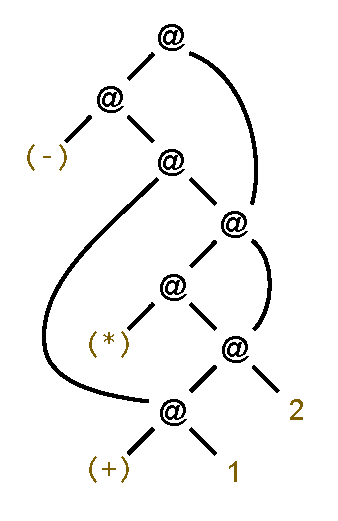
\includegraphics[scale=0.5]{images/sec-5/sharing-original}
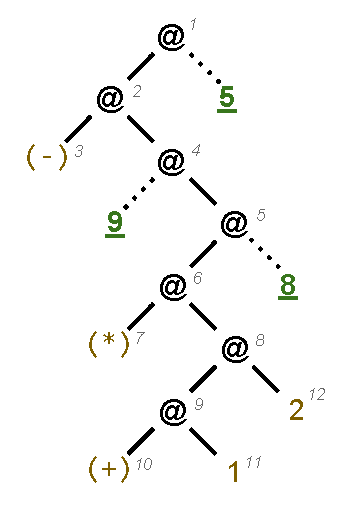
\includegraphics[scale=0.5]{images/sec-5/sharing-pruned}
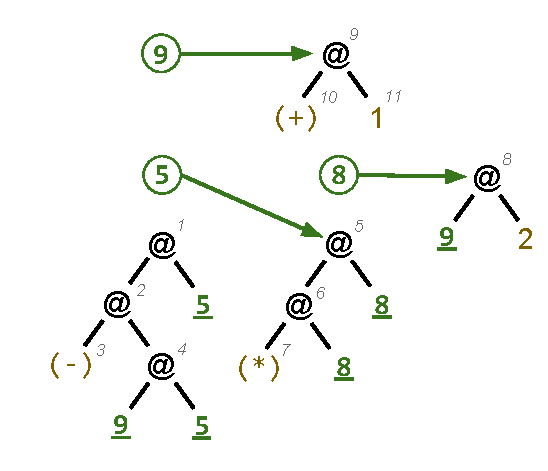
\includegraphics[scale=0.5]{images/sec-5/sharing-floated}
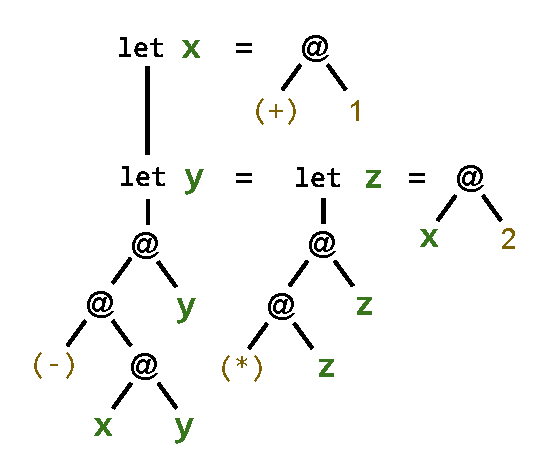
\includegraphics[scale=0.5]{images/sec-5/sharing-lets}
\caption{Recovering sharing in an example term}
\label{fig:sharing_recovery}
\end{figure}

The contribution of the sharing recovery algorithm is work done primarily by my
supervisor Manuel Chakravarty, so I present here only a brief overview of the
method; see \cite{McDonell:2013wi} for details. Consider the following source
term:
%
\begin{lstlisting}
let inc = (+1) 1
in let nine = let three = inc 2
              in
              (*) three three
in
(-) (inc nine) nine
\end{lstlisting}
%
The term's abstract syntax DAG is shown as the left-most diagram in
Figure~\ref{fig:sharing_recovery}, which uses \app\ nodes to represent
application. Typed conversion from HOAS with sharing recovery proceeds in three
stages:


\subsubsection*{Phase 1: Prune shared terms:}

A depth-first traversal of the AST\index{abstract syntax tree} annotates each node
with its unique stable name\index{stable name}, and builds an occurrence map for
the number of times we see each node in the overall program. The stable names of
two Haskell terms are equal only when the terms are represented by the same heap
structure in memory. Likewise, when the abstract syntax tree of two terms of an
embedded language program have the same stable name, we know that they represent
the same value. If we encounter a node already in the occurrence map, it
represents a previously visited node and is thus a \emph{shared subterm}. We
replace the entire subterm at that node with a placeholder containing its stable
name. The second diagram in Figure~\ref{fig:sharing_recovery} shows the outcome
of this stage. Each node is labelled by a number that represents its stable name,
and the dotted edges indicate where we encountered a previously visited, shared
node. The placeholders are indicated by underlined stable names. In this way all
but the first occurrence of a shared subterm are pruned
%and replaced with variable bindings,
so that we do not descend into terms that have been previously encountered. This
avoids completely unfolding the embedded expression, so the complexity of
sharing observation is proportional to the number of nodes in the tree
\emph{with} sharing.

As the stable name of an expression is an intensional property, it can only be
determined in Haskell's @IO@ monad, and strictly speaking because of this
it is not deterministic. The stable name API does not guarantee completeness:
for two stable names @sn1@ and @sn2@, if @sn1 == sn2@ then the
two stable names were created from the same heap object. However, the reverse is
not necessarily true; if the two stable names are not equal the objects they
come from may still be equal. Put another way, equality on stable names may
return a false negative, which means that we fail to discover some sharing, but
can never return a false positive since stable names from different heap objects
are not considered equal. Luckily, sharing does not affect the denotational
meaning of the program, and hence a lack of sharing does not compromise
denotational correctness.


\subsubsection*{Phase 2: Float shared terms:}

A bottom-up traversal that determines the scope for every binding to be
introduced to share a subterm. It uses the occurrence map to determine, for
every shared subterm, the meet of all the shared subterm occurrences --- the
lowest AST node at which the binding for the subterm can be placed. This is why
the occurrence map generated in the previous phase can not be simplified to a
set of occurring names: we need the actual occurrence count to determine where
shared subterms should be let-bound.

The third diagram of Figure~\ref{fig:sharing_recovery} shows the result of this
process. Floated subterms are referenced by circled stable names located
\emph{above} the node that they floated to. If the node collects more than one
shared subterm, the subterm whose origin is deeper in the original term goes on
top; here, 9 on top of 5. Nested sharing leads to subterms floating up inside
other floated subterms; here, 8 stays inside the subterm rooted at 5.


\subsubsection*{Phase 3: Binder introduction:}

Finally, each floated subterm gets let-bound right above the node it floated to,
as shown in the rightmost diagram of Figure~\ref{fig:sharing_recovery}. At the
same time, the AST is converted into nameless \indext{de Bruijn} form by
introducing de Bruijn indices at the same time as introducing the lets.


\section{Common subexpression elimination}
\label{sec:cse}

\emph{Common subexpression elimination} finds computations that are performed at
least twice on a given execution path and eliminates the second and later
occurrences, replacing them with uses of saved values. The current
implementation performs a simplified version of common subexpression
elimination, where we look for expressions of the form:
%
\begin{lstlisting}[style=Haskell,numbers=none]
%\bf$\langle$ common subexpression elimination $\rangle$% let x = e1 in [x/e1]e2
\end{lstlisting}
%
and replace all occurrences of @e1@ in @e2@ with @x@. This method relies on the
introduction of let-bindings into the reified program by the sharing recovery
algorithm, described in the previous section (\S\ref{sec:sharing_recovery}), so
can not eliminate any common subexpressions that are not already defined in the
source program. Thus, the method might not completely eliminate all redundant
expressions from the program, but is sufficient to catch some cases, in
particular those that tend to be introduced during the array fusion
optimisation, described in the following section.
%\footnote{\url{http://hackage.haskell.org/trac/ghc/ticket/701}}

While it may seem that common subexpression elimination is always worthwhile, as
it reduces the number of arithmetic operations performed, this is not
necessarily advantageous. The simplest case in which it may not be desirable is
if it causes a register to be occupied for a long time in order to hold the
shared expression's value, which hence reduces the number of registers available
for other uses. Even worse is if that value has to be spilled to memory because
there are insufficient registers available, or if the number of active threads
is too low to be able to hide global memory access latency
(\S\ref{sec:thread_occupancy}). Investigation of this tricky target-dependent
issue is left for future work.


\section{Array fusion}
\label{sec:array_fusion}

Fusion, or deforestation, is a term used to describe techniques for having a
compiler automatically eliminate intermediate data structures in a computation
by combining successive traversals over these data structures. For example, to
compute the sum of squares of all integers from one to a given number in
Haskell~\cite{Haskell:1998}, one could write:
%
\begin{lstlisting}[style=haskell]
sum_of_squares :: Int -> Int
sum_of_squares n
    = sum                       -- add all numbers in the list
    $ map (\x -> x * x)         -- traverse list doubling each element
    $ enumFromTo 1 n            -- generate list of numbers [1..n]
\end{lstlisting}
%
While the meaning of the program is clear, it is inefficient, as this code
produces two intermediate lists of numbers which each require $O(n)$ memory to
store and data transfers to manipulate. Instead, one could write the program
as a single tail-recursive loop as such:
%
\begin{lstlisting}[style=haskell]
sum_of_squares :: Int -> Int
sum_of_squares n = go 1 0
  where
    go i acc | i > n     = acc                   -- return final tally
             | otherwise = go (i+1) (acc + i*i)  -- add to accumulator and step to next element
\end{lstlisting}
%
The second program is much more efficient than the first because it does not
involve the production of any intermediate lists and executes is constant space.
Unfortunately, the clarity of the original program has been lost. What we
\emph{really} want is to write the first program, and have the compiler
\emph{automatically} transform it into the second, or something morally
equivalent.

This example also demonstrates a subtle behavioural tendency of optimising
program transformations: while the second (target) program does not produce any
intermediate data structures as desired, we can no longer interpret the program
as a sequence of combinators, such as @map@ and @sum@. This observation is
critical if the combinators represent collective operations expressed as
algorithmic skeletons, as they do in Accelerate: while the second program
compiles to an efficient \emph{scalar} loop, its \emph{parallel} interpretation
has been lost.


\subsection{Considerations}

Fusion in a massively data-parallel (embedded) language such as Accelerate
requires several uncommon considerations. We discuss related work further in
section~\ref{sec:fusion_related_work}.

\paragraph{Parallelism:} While fusing parallel collective operations, we must be
careful not to lose information essential to parallel execution. For example,
@foldr/build@\index{fusion!foldr/build}~\cite{Gill:1993de} and
stream\index{fusion!stream}~\cite{Coutts:2007kp} fusion are not applicable,
because they produce sequential tail-recursive loops rather than massively
parallel GPU kernels. Similarly the
@split/join@\index{fusion!split/join}~\cite{Keller:1999ic} approach used by
DPH\index{data-parallel Haskell} is not helpful. Although fused operations are
split into sequential and parallel subcomputations, the granularity of the
parallel operations is rather coarse and the sequential component again consists
of tail-recursive loops, both of which are ill suited for a massively parallel
target such as GPUs. Accelerate compiles massively parallel array combinators to
CUDA code via template skeleton instantiation~(\S\ref{sec:code_generation}), so
any fusion system must preserve the combinator representation of the
intermediate code.


\paragraph{Sharing:} \index{fusion!short-cut}Short-cut fusion transforms rely on
inlining to move producer and consumer expressions next to each other, which
allows adjacent constructor/destructor pairs to be detected and eliminated. When
let-bound variables are used multiple times in the body of an expression,
unrestrained inlining can lead to duplication of work. Compilers such as GHC
handle this situation by inlining the definitions of let-bound variables that
have a single use site, or by relying on some heuristic about the size of the
resulting code to decide what to inline~\cite{PeytonJones:2003gb}. In typical
Accelerate programs, each array is used at least twice: once to access the shape
information and once to access the array data, so we must handle at least this
case specially.

\paragraph{Fusion at runtime:} As the Accelerate language is embedded in
Haskell, compilation of the Accelerate program happens at Haskell \emph{runtime}
rather than when compiling the Haskell
program~(\S\ref{sec:dynamic_compilation}). For this reason, optimisations
applied to an Accelerate program contribute to its overall runtime, so we must
be mindful of the cost of analysis and code transformations. On the flip-side,
we are able to make use of information that is only available at runtime.

\paragraph{Filtering:} General array fusion transformations must deal with
filter-like operations, for which the size of the result structure depends on
the \emph{values} of the input array, as well as its size. For example
\index{fusion!stream}stream fusion includes the @Skip@ constructor in
order to support filtering operations (among other uses). Although easily
implementable as a combination of the core primitives and provided by the
library as such, filtering is difficult to implement as a single-step parallel
operation. Since filter-like operations are not part of the core Accelerate
operations, we do not need to consider them further.

% Today I did some of my thesis. I wrote LOOOOOTS of pages of words and thingies.
% I think I should get to have ALLLLL the plays and ALLLLLL the rests now. Thesis,
% you are STOOOOPID. WHy can't you write yourself? Huh? Everyone else provides for
% themself, so why don't you! DOn't turn this against me and say that writing my
% thesis is me providing for myself. YOU THIK I DONT KNOW WHAT. Stupid thesis.
% Go home.
% LET'S FUCK!
%
%   - pookie 19/06/2013

\paragraph{Fusion on typed de Bruijn indices:} We fuse Accelerate programs by
rewriting typed \indext{de Bruijn} terms in a type preserving manner.
Maintaining type information adds complexity to the definitions and rules, but
amounts to a partial proof of correctness checked by the type checker
(\S\ref{sec:richly_typed_terms}).


\subsection{The Main Idea}
\label{sec:the_main_idea}

All collective operations in Accelerate are array-to-array transformations.
Reductions, such as @fold@, which reduce an array to a single element,
yield a singleton array rather than a scalar expression. We partition array
operations into two categories:

\begin{enumerate}
    \item Operations where each element of the result array depends on (at most)
        one element of each input array. Multiple elements of the output array
        may depend on a single input array element, but all output array
        elements can be computed independently. We refer to these operations as
        \index{producer}\emph{producers}.

    \item Operations where each element of the result array depends on multiple
        elements of the input array. We call these operations
        \index{consumer}\emph{consumers}, in spite of the fact that, as with all
        collective operations in Accelerate, they also produce an array as
        output.
\end{enumerate}

\begin{lstlisting}[
    style=haskell_float,
    numbers=none,
    float=t,
    label={lst:producer_consumer_operations},
    caption={[Producer and consumer operations in Accelerate] Summary of Accelerate's core
        collective array operations, classified as either producer of consumer
        operations. We omit the \code{Shape} and \code{Elt} class constraints
        for brevity. In addition, there are other flavours of folds and scans as
        well as segmented versions of these.}]
%\makebox[\textwidth]{\rm\bf Producers}%

map         :: (Exp a -> Exp b) -> Acc (Array sh a)                   %\rm map a function over an array%
            -> Acc (Array sh b)
zipWith     :: (Exp a -> Exp b -> Exp c) -> Acc (Array sh a)          %\rm apply funciton to a\ldots%
            -> Acc (Array sh b) -> Acc (Array sh c)                   %\rm \ldots pair of arrays%

backpermute :: Exp sh' -> (Exp sh' -> Exp sh) -> Acc (Array sh a)     %\rm backwards permutation%
            -> Acc (Array sh' e)
replicate   :: Slice slix                                             %\rm extend array across\ldots%
            => Exp slix -> Acc (Array (SliceShape slix) e)            %\rm \ldots new dimensions%
            -> Acc (Array (FullShape slix) e)
slice       :: Slice slix                                             %\rm remove existing dimensions%
            => Acc (Array (FullShape  slix) e) -> Exp slix
            -> Acc (Array (SliceShape slix) e)
reshape     :: Exp sh' -> Acc (Array sh e) -> Acc (Array sh' e)       %\rm reshape an array%

generate    :: Exp sh -> (Exp sh -> Exp a) -> Acc (Array sh a)        %\rm array from index mapping%

%\makebox[\textwidth]{\rm\bf Consumers}%

fold        :: (Exp a -> Exp a -> Exp a) -> Exp a                     %\rm tree reduction along\ldots%
            -> Acc (Array (sh:.Int) a) -> Acc (Array sh a)            %\rm \ldots innermost dimension%
scan{l,r}   :: (Exp a -> Exp a -> Exp a) -> Exp a -> Acc (Vector a)   %\rm left-to-right or right-to-left%
            -> Acc (Vector a)                                         %\rm \ldots vector pre-scan%
permute     :: (Exp a -> Exp a -> Exp a) -> Acc (Array sh' a)         %\rm forward permutation%
            -> (Exp sh -> Exp sh') -> Acc (Array sh a)
            -> Acc (Array sh' a)
stencil     :: Stencil sh a stencil => (stencil -> Exp b)             %\rm map a function with local\ldots%
            -> Boundary a -> Acc (Array sh a) -> Acc (Array sh b)     %\rm \ldots neighbourhood context%
\end{lstlisting}

Listing~\ref{lst:producer_consumer_operations} summarises the collective array operations that we
support. In a parallel context, producers are much more pleasant to deal with
because independent element-wise operations have an obvious mapping to massively
parallel processors such as GPUs\index{graphics processing unit}. Consumers are
a different story, as we need to know exactly how the elements depend on each
other in order to implement them efficiently in parallel. For example, a
reduction (with associative operator) can be implemented efficiently in
parallel as a recursive tree reduction (\S\ref{sec:parallel_reduction}), but a
parallel scan requires two distinct phases (\S\ref{sec:parallel_scan}).
Unfortunately, this is the sort of information that is obfuscated by most fusion
techniques (\S\ref{sec:fusion_related_work}). To support the different
properties of producers and consumers, the fusion transform is split into two
distinct phases:
%
\begin{enumerate}
    \item \emph{Producer/producer:} A bottom-up contraction of the AST that
        fuses sequences of producers into a single producer. This is implemented
        as a source-to-source transformation on the \index{abstract syntax
        tree}AST\@.

    \item \emph{Producer/consumer:} A top-down transformation that annotates the
        AST as to which nodes should be computed to manifest data and which
        should be embedded into their consumers. This process is ultimately
        completed during code generation, where we specialise the consumer
        skeleton by directly embedding the code for producing each element into
        the skeleton.

\end{enumerate}

\begin{figure}[htb]
    \flushright \small(Before fusion)\qquad\\
    \centering  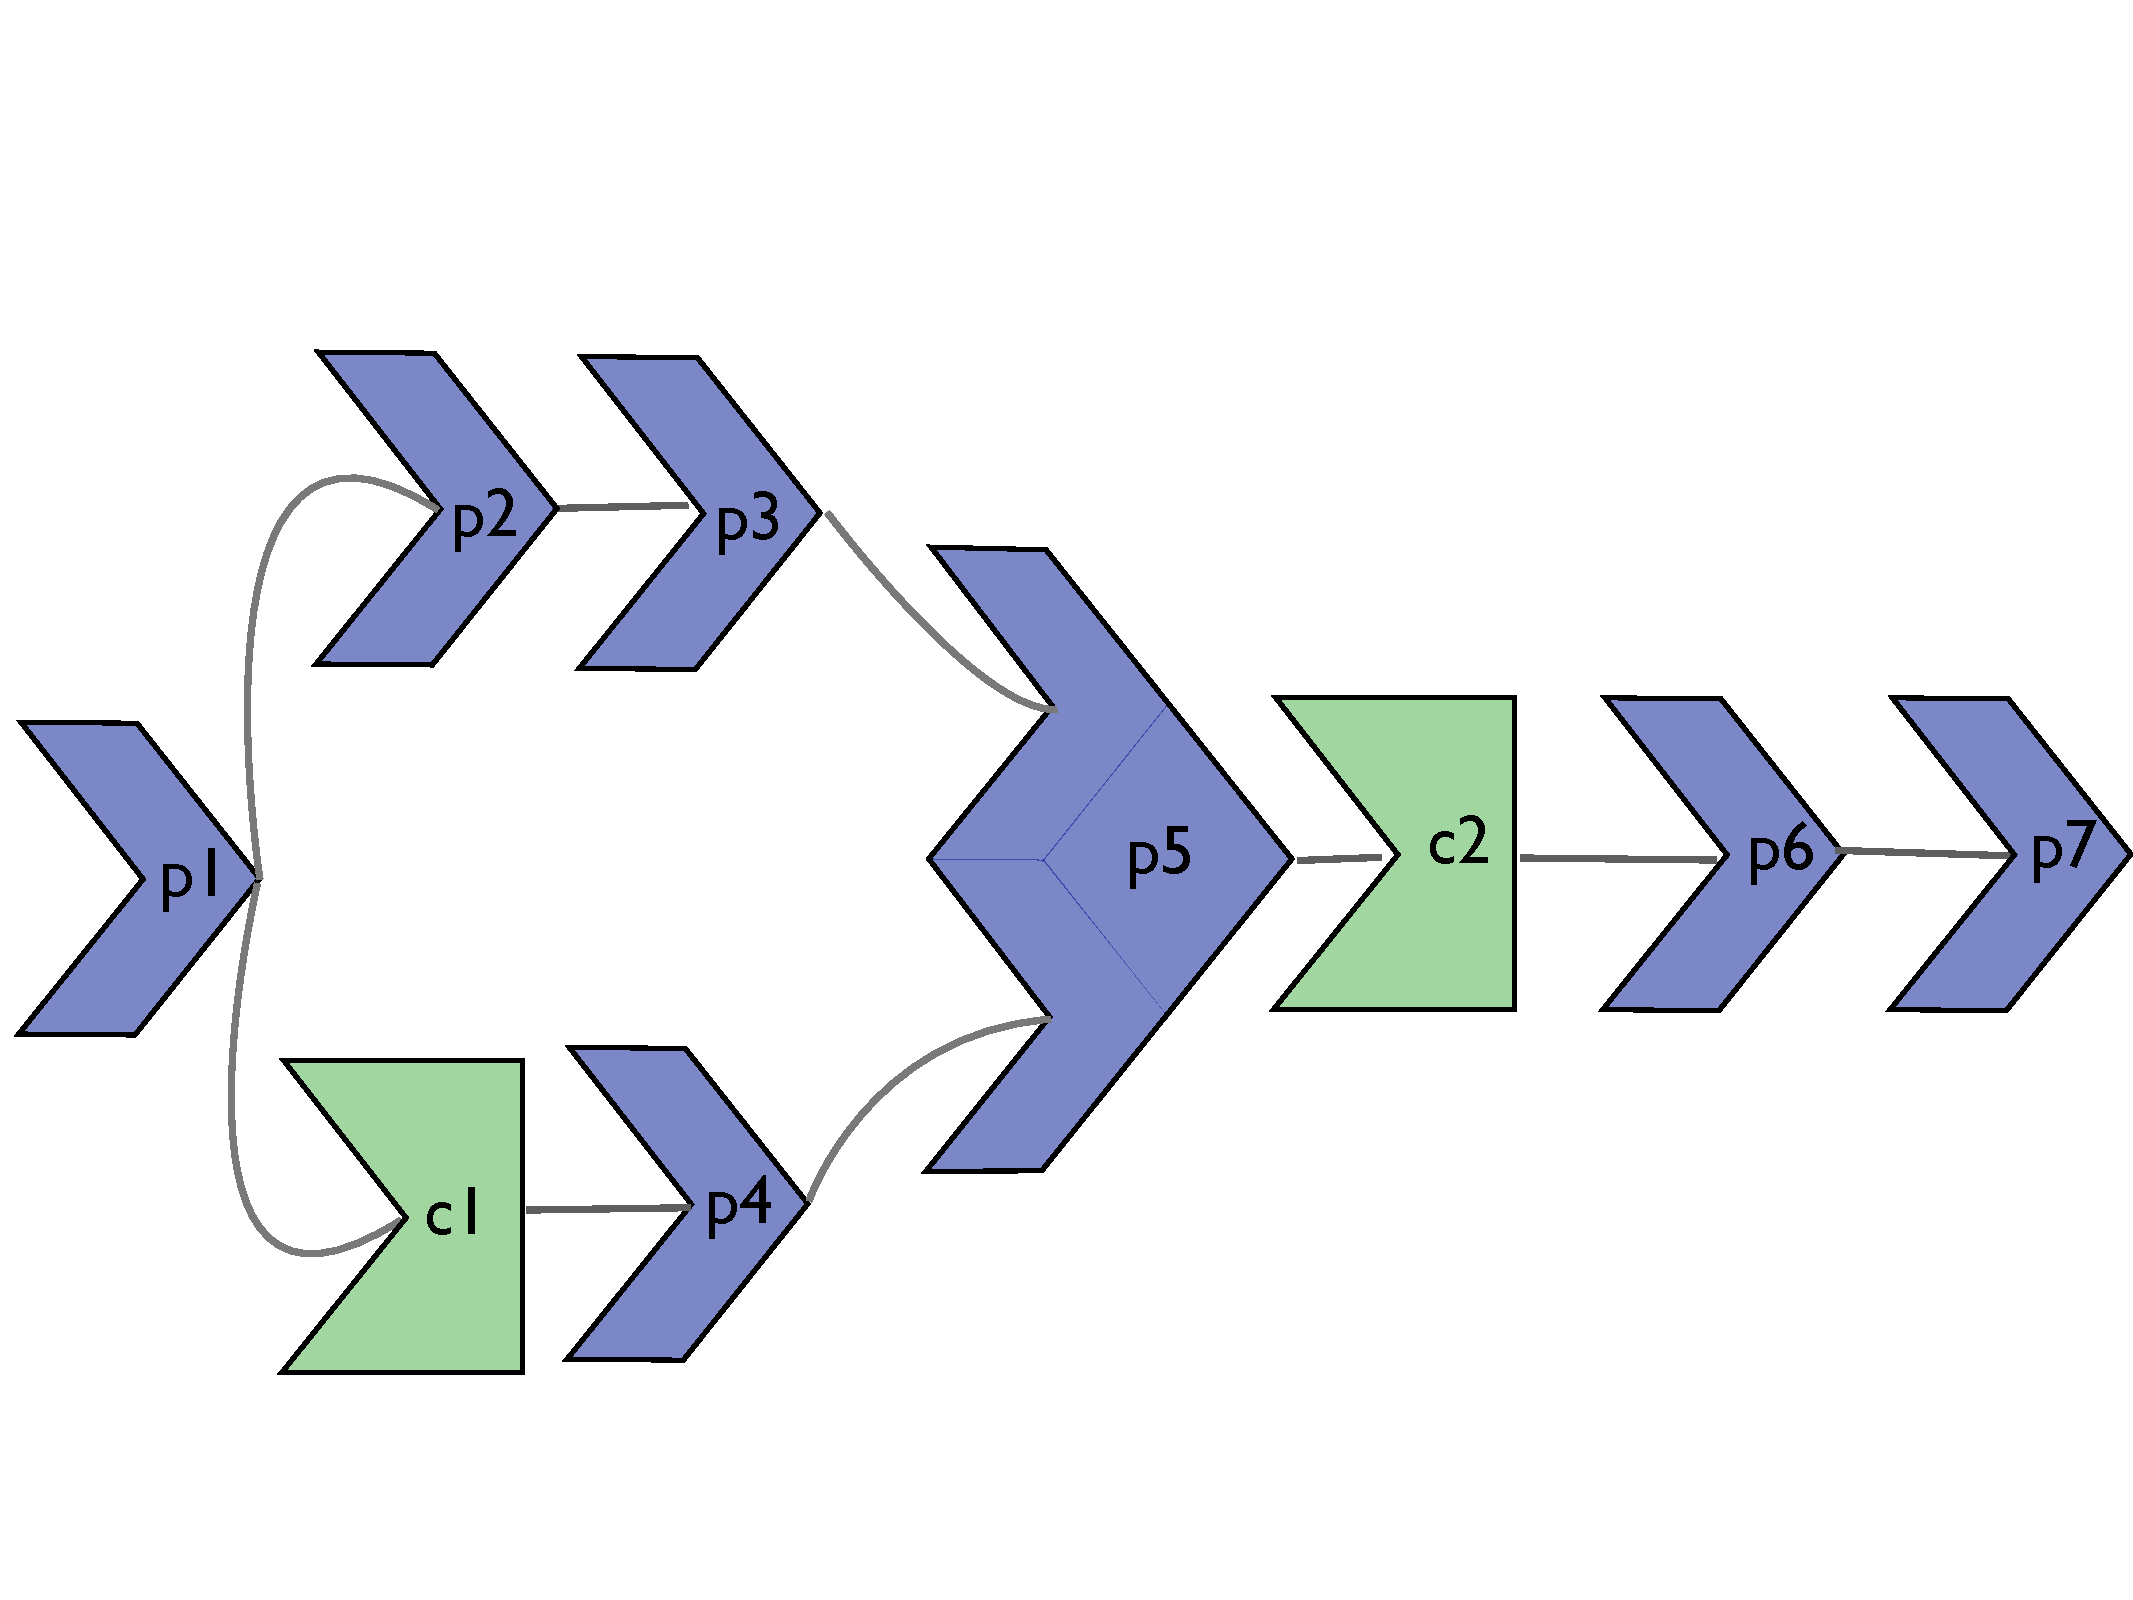
\includegraphics[scale=0.25]{images/sec-5/fusion1.pdf}
    \flushright \small(After producer/producer fusion)\qquad\\
    \centering  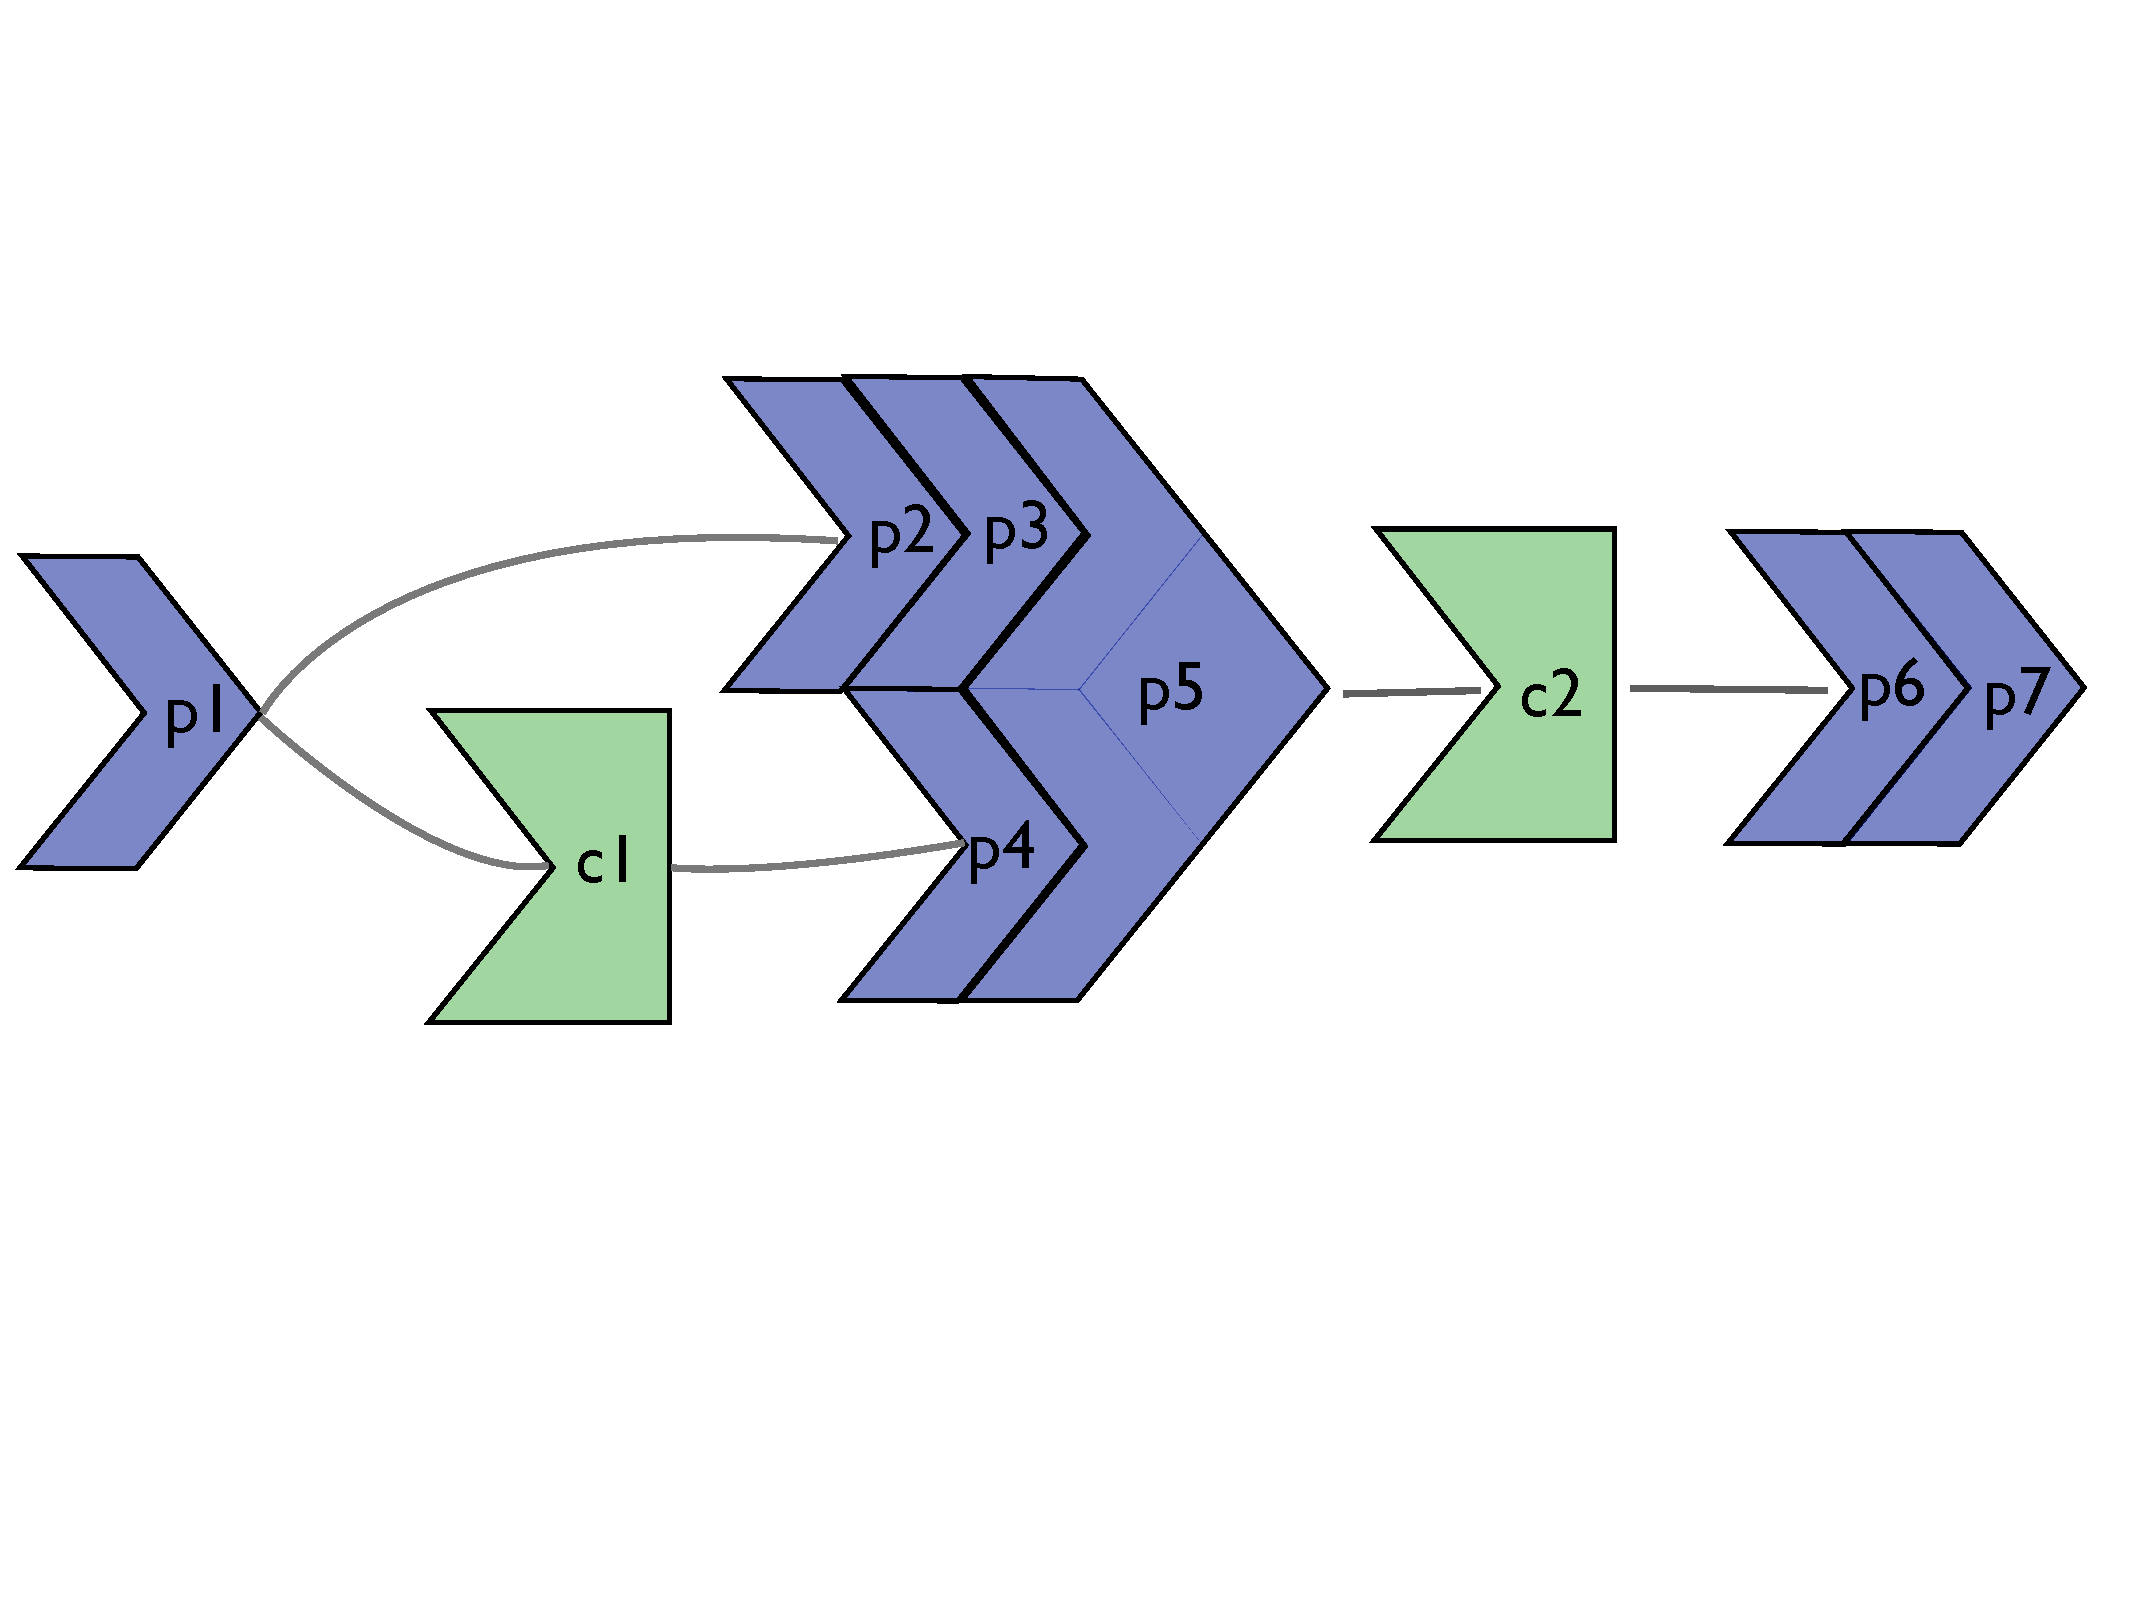
\includegraphics[scale=0.25]{images/sec-5/fusion2.pdf}
    \flushright \small(After producer/consumer fusion)\qquad\\
    \centering  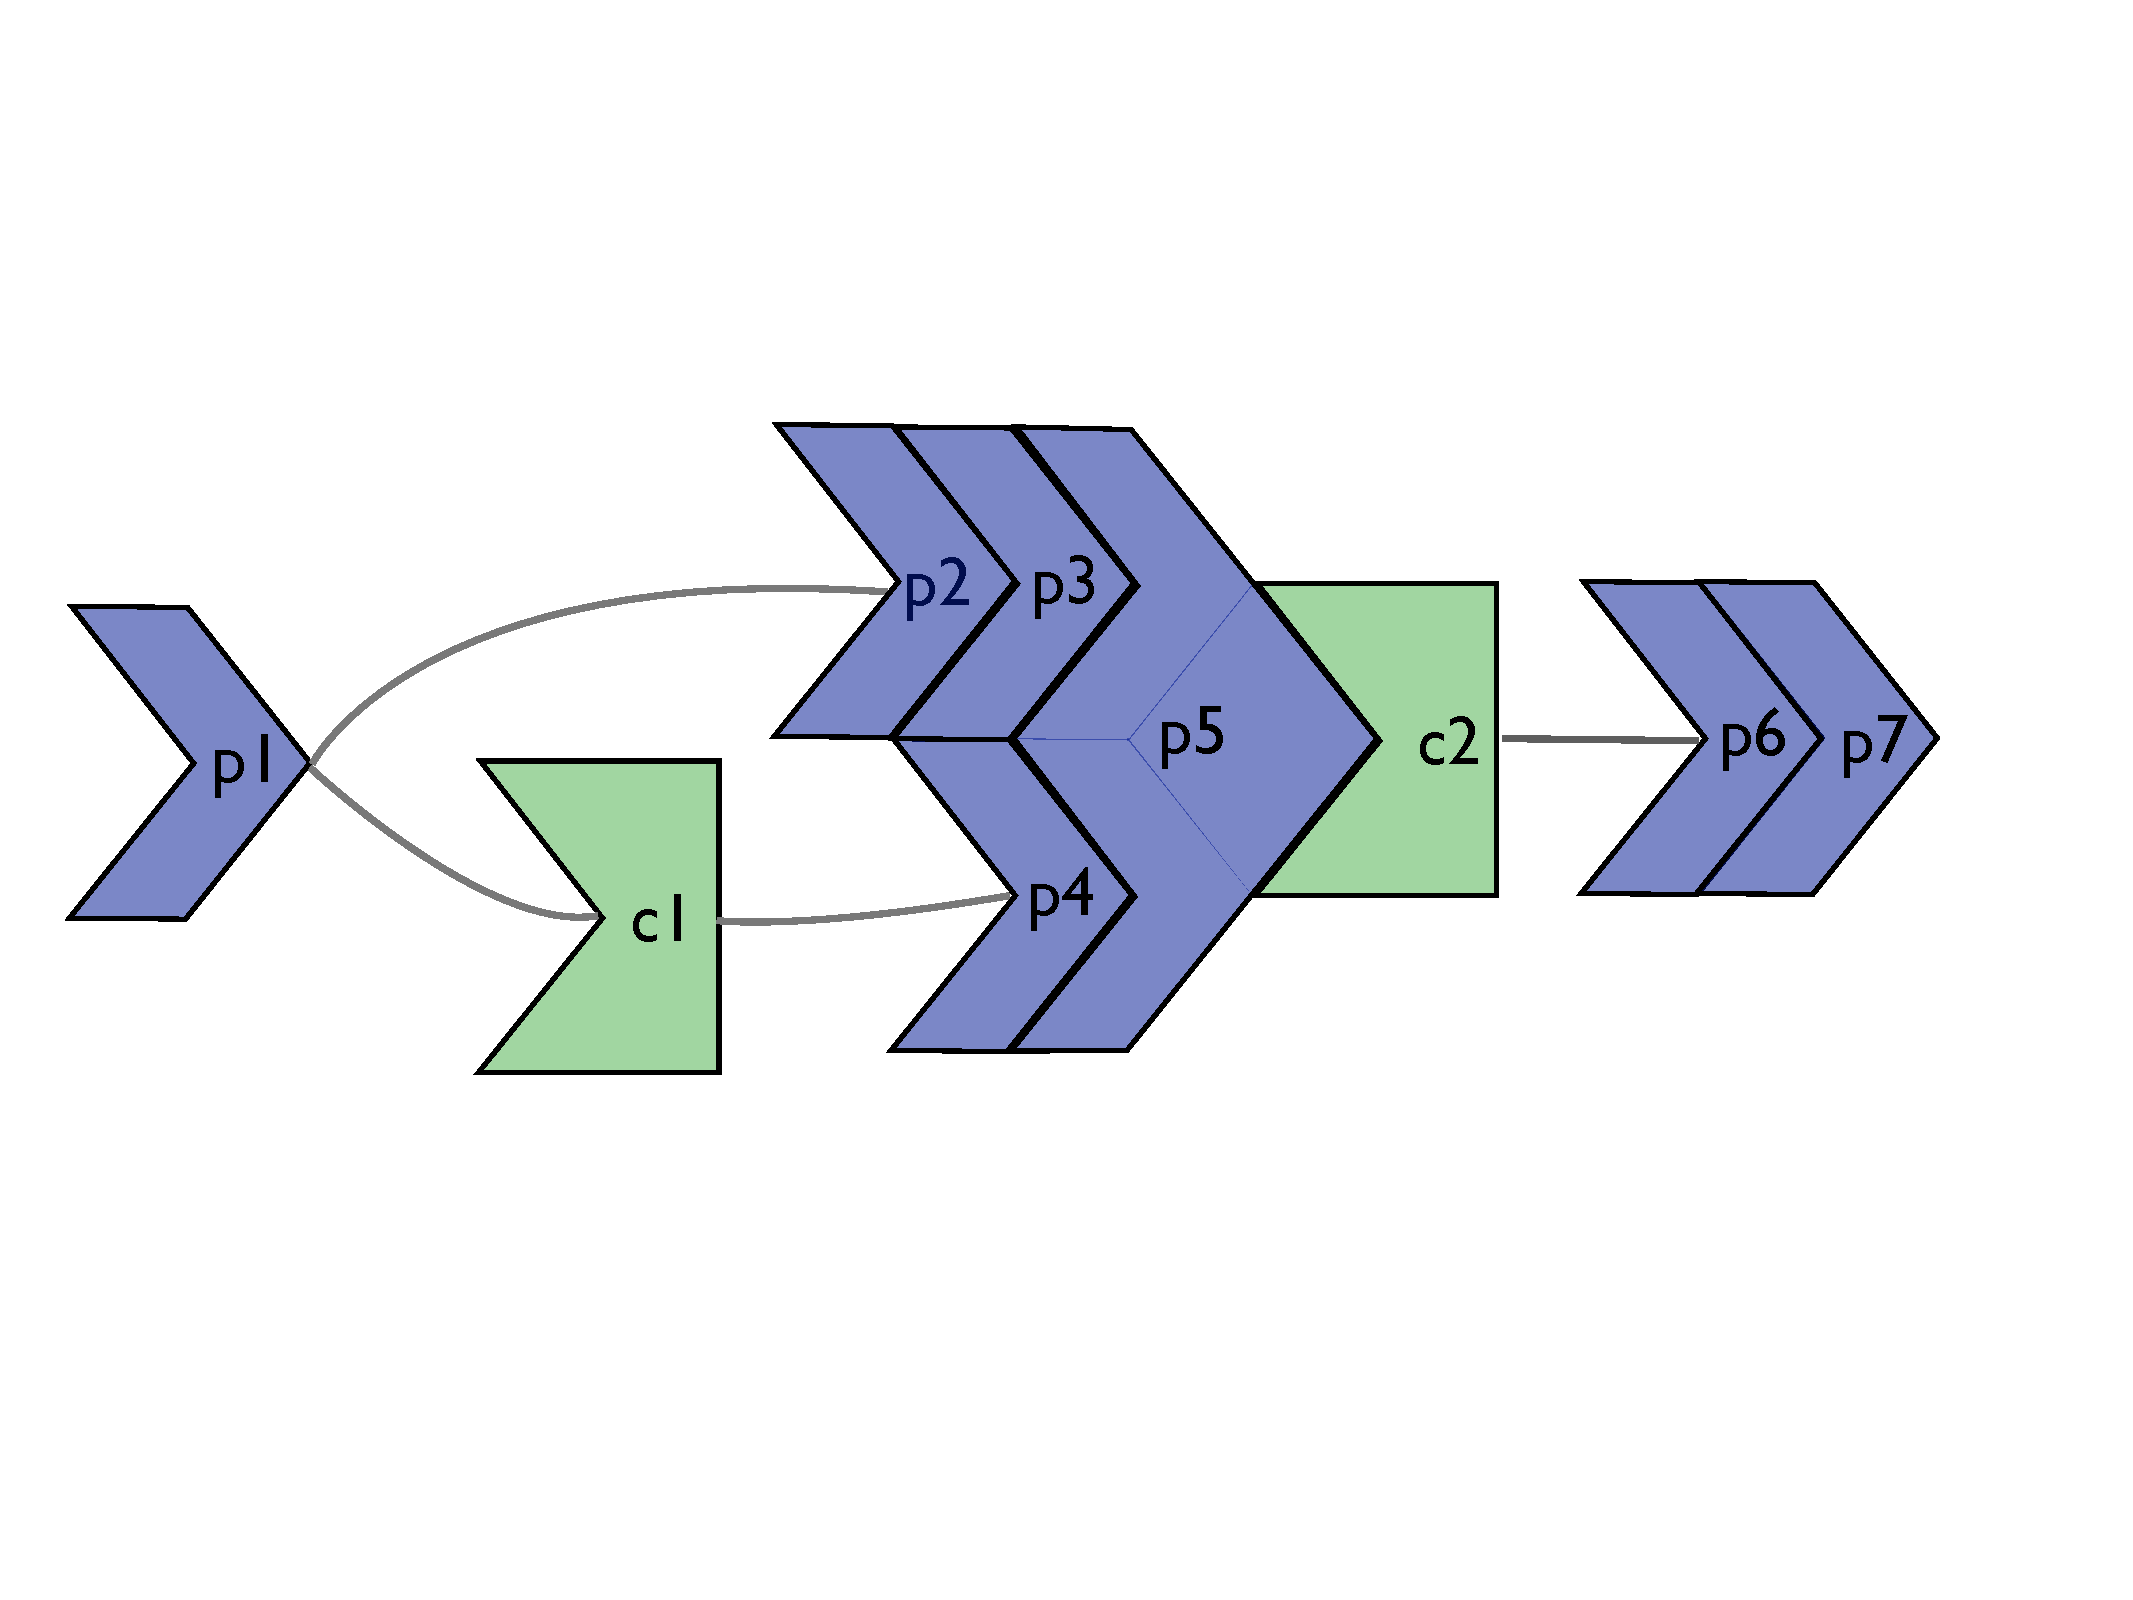
\includegraphics[scale=0.25]{images/sec-5/fusion3.pdf}
    \caption[Fusion in Accelerate]{Producer/producer and Producer/consumer fusion in Accelerate.}
    \label{fig:fusion}
\end{figure}

Figure~\ref{fig:fusion} shows how the fusion technique affects the
AST\index{abstract syntax tree}: blue boxes labelled $p_1$ to $p_7$ represent
producers, where $p_5$ is a producer like @zipWith@ that takes two arrays
as input. The consumers are labelled $c_1$ and $c_2$. In the first phase all
adjacent producers are fused, with the exception of $p_1$ whose result is used
by both $c_1$ and $p_2$. In the second phase, the fused producers are embedded
into consumers where possible.

Throughout the transformation $p_1$ is left as is, as its result is used by both
$c_1$ and $p_2$. It would be straightforward to change the implementation such
that the work of $p_1$ is duplicated into both $p_2$ and $c_1$. Despite reducing
memory traffic, this is not always advantageous, so the current implementation
is conservative and never duplicates work. Since Accelerate is a restricted,
deeply embedded language, we can compute accurate cost estimates and make an
informed decision, but this is left for future work. Moreover, this is an
instance of a fundamental limitation with \index{fusion!short-cut}short-cut
fusion techniques such as
\index{fusion!foldr/build}@foldr/build@~\cite{Gill:1993de} and
\index{fusion!stream}stream~\cite{Coutts:2007kp} fusion. Since short-cut fusion
is a local transformation that depends on inlining, it is applicable only to
fusing operations which have a single use site. To implement fusion where an
array is efficiently consumed by multiple operations without work duplication
would require fundamental changes to the algorithm.
%
Producer/consumer fusion of $c_1$ into $p_4$, or $c_2$ into $p_6$, would also
require substantial changes to the fusion implementation.


\section{Implementing array fusion}
\label{sec:implementing_array_fusion}

As we saw in Figure~\ref{fig:fusion}, the main idea is that successive producer
operations are fused together ($p_2$, $p_3$, $p_4$ and $p_5$), and producers are
fused into consumers ($p_{ 2,3,4,5 }$ into $ c_2$). The current implementation
do not fuse the results of consumers into subsequent producers ($c_2$ is not
fused into $p_{ 6,7 }$), and producers used multiple times ($p_1$) are not fused
either.
% This has the happy consequence of maintaining trickiest parts of the parallel
% interpretation of the program.

We require a representation that will facilitate embedding fused producer
terms into consumers. We do not wish to manipulate source terms directly, as
this would require a number of rewrite rules quadratic in the number of
operations that are to be fused. This was the problem with Wadler's original
deforestation algorithm~\cite{Wadler:1981hy,Wadler:1990ix}. The representation
must also be sufficiently expressive to represent all operations we want to
fuse, which was a limitation of \index{fusion!foldr/build}@foldr/build@
fusion~\cite{Gill:1993de}.


\subsection{Representing Producers}
\label{sec:representing_producers}

The basic idea behind the representation of producer arrays in Accelerate is
well known: simply represent an array by its size and a function mapping array
indices to their corresponding values. This method has been used successfully to
optimise purely functional array programs in \index{fusion!delayed
arrays}Repa~\cite{Keller:2010er}, and has also been used by
others~\cite{Claessen:2012hl}.

The use of delayed arrays in Repa was originally motived by the desire to avoid
superfluous copying of array elements during index space transformations such as
@backpermute@ (see Listing~\ref{lst:producer_consumer_operations}). Another
major benefit of delayed arrays is that it offers by-default automatic fusion.
Moreover, this fusion does not require sophisticated compiler transformations or
for the two fusible terms to be statically juxtaposed; fusion is a property of
the data representation.

Automatic fusion sounds too good to be true, and indeed it is. There are at
least two reasons why it is not always beneficial to represent all array terms
uniformly as functions. The first issue is \emph{sharing}. Consider the
following:
%
\begin{lstlisting}[style=haskell]
let b = map f a
in  mmMult b b
\end{lstlisting}
%
Every access to an element @b@ will apply the (arbitrarily expensive)
function @f@ to the corresponding element of @a@. It follows that
these arbitrarily expensive computations will be done \emph{at least twice},
once for each argument of @mmMult@, quite contrary to the programmer's
intent. Indeed, if @mmMult@ consumes its elements in a non-linear manner,
accessing elements more than once, the computation of @f@ will be performed
every time. We must be able to represent some terms as manifest arrays so that a
delayed-by-default representation can not lead to an arbitrary loss of sharing.
This is a well known problem with Repa~\cite{Lippmeier:2012g}.

The other consideration is \emph{efficiency}. Since we are targeting a massively
parallel architecture designed for performance, it is better to use more
specific operations whenever possible. An opaque indexing function is too
general, conveying no information about the pattern in which the underlying
array is accessed, and hence no opportunities for optimisation.

Listing~\ref{lst:cunctation} describes the ways in which the fusion
transformation represents intermediate arrays. The fusion process operates by
recasting producer array computations in terms of a set of scalar functions used
to construct an element at each index, % encoded by this data structure, and
fusing successive producers by combining these scalar functions.
%
\begin{lstlisting}[style=haskell_float
    ,label=lst:cunctation
    ,caption={Representation of fusible producer arrays}]
data Cunctation acc aenv a where
    Done  :: Arrays arrs
          => Idx            aenv arrs                   -- manifest array(s)
          -> Cunctation acc aenv arrs

    Yield :: (Shape sh, Elt e)
          => PreExp     acc aenv sh                     -- output shape
          -> PreFun     acc aenv (sh -> e)              -- compute an element at each index
          -> Cunctation acc aenv (Array sh e)

    Step  :: (Shape sh, Shape sh', Elt a, Elt b)
          => PreExp     acc aenv sh'                    -- output shape
          -> PreFun     acc aenv (sh' -> sh)            -- backwards permutation into input array
          -> PreFun     acc aenv (a   -> b)             -- function to apply to input value
          -> Idx            aenv (Array sh  a)          -- manifest input array
          -> Cunctation acc aenv (Array sh' b)
\end{lstlisting}
%
\makeatchar
The representation\footnote{%
cunc$\cdot$ta$\cdot$tion
\textcolor{gray}{|
k\textipa{`}NGk\textquotesingle t\={a}SH\textipa{`}n \enspace\textipa{k@Nk}\textquotesingle \textipa{te\;IS@n}
% kəNGkˈtāSHən\enspace kəŋkˈteɪʃən
|} (n) the action or an instance of delaying; tardy action.}
\makeatcode
%
is parameterised by the recursive closure of array computations @acc@, the
array environment @aenv@, and has three constructors:
%
\begin{enumerate}
\item @Done@ injects a manifest array into the type.
    %represented as a reference to a term in the array environment.

\item @Yield@ defines a new array in terms of its shape and a function
    that maps indices to elements.

\item @Step@ encodes a special case of @Yield@, that defines a new
    array by applying an index and value transformation to an argument array.

\end{enumerate}

Note that the argument arrays to @Done@ and @Step@ are not expressed as terms in
@acc@, the type of collective array operations. Instead, requiring a \indext{de
Bruijn} index (@Idx@) into the array environment ensures that the argument array
is manifest. Thus the definition of @Cunctation@ is non-recursive in the type of
array computations. This allows the representation to be (later) embedded within
producer terms (\ref{sec:producer_consumer_fusion}) with the guarantee that an
embedded scalar computation will not invoke further parallel computations
(\S\ref{sec:array_computations_vs_scalar_expressions}).
% \footnote{While scalar expression terms are mutually recursive in
% \footcode{acc}, we are guaranteed that these terms will consist only of free
% array variables (\footcode{Idx}).}

In order to bring additional array terms into scope, which may be required for
@Done@ and @Step@, we combine this representation of producer arrays with the
method of section~\ref{sec:environment_manipulation} for collecting
supplementary environment bindings. Listing~\ref{lst:Embed} shows the complete
data structure used for representing producer terms in Accelerate.
%
\begin{lstlisting}[style=haskell_float
    ,label=lst:Embed
    ,caption={Representation of fused producer arrays in Accelerate}]
data Embed acc aenv a where
    Embed :: Extend     acc aenv aenv'      -- additional bindings to bring into scope, to evaluate the\ldots
          -> Cunctation acc      aenv' a    -- \ldots representation of (fused) producer terms
          -> Embed      acc aenv       a
\end{lstlisting}

Note the types of the array environments in Listing~\ref{lst:Embed}. The @Embed@
type is expressed in relation to the type @aenv@, which represents all
let-bindings currently in scope at this point of the AST\index{abstract syntax
tree} that we are analysing. The data constructor contains an
existentially typed @aenv'@. This existential is witnessed by the first argument
@Extend@, that contains any additional array terms collected during the fusion
process (\S\ref{sec:environment_manipulation}). The delayed array representation
in the second argument is expressed in terms of this extended environment, so
has access to any terms from the AST (@aenv@) as well as those additional
bindings introduced by @Extend@ (@aenv'@).

Why do we separate the auxiliary bindings from the representation of fused
producers? The constructors of @Cunctation@ could carry this information,
and then we would not require this additional data structure. For example, the
following is a valid alternative definition for the @Yield@ constructor:
%
\begin{lstlisting}[style=haskell]
  Yield' :: (Shape sh, Elt e)                   -- Alternative definition (bad)
         => Extend     acc aenv aenv'           -- NEW: supplementary environment bindings
         -> PreExp     acc      aenv' sh        -- CHANGED: terms now defined w.r.t. \texttt{aenv'}
         -> PreFun     acc      aenv' (sh -> e)
         -> Cunctation acc aenv       (Array sh e)
\end{lstlisting}

To create a real AST\index{abstract syntax tree} node from the @Embed@
representation, we need both the environment bindings as well as the array
description. However, analysis of how to fuse terms requires only the array
description. If the additional bindings are bundled as part of the array
representation, as in @Yield'@, the existentially quantified environment
type is only available after we pattern match on the constructor. This is
problematic because to inspect terms and do things like function composition
(\S\ref{sec:function_composition}) the types of the environments of the two
terms must be the same, so after we pattern match on the constructor we must
@sink@ (\S\ref{sec:sinking}) the second term into @aenv'@. Even worse,
for terms in the delayed state the only way to do this sinking is to first
convert them into a real AST node and then back into the delayed state. If for
some reason we can not fuse into this representation --- for example we do not
meet the requirements for the more restrictive @Step@ --- then this
additional work is wasted.

Why can we not analyse terms with respect to the exposed environment type
@aenv@, ignoring for the moment the existential? At some point we will need
to combine the extended environments, and we have no way to do this even if the
existential types are exposed.
%
\begin{lstlisting}[style=haskell]
cat :: Extend env env1 -> Extend env env2 -> Extend env ???
\end{lstlisting}

Because of the limited scope in which the existential type is available in the
@Yield'@ style representation, we ultimately perform this process of converting
terms and sinking into a suitable type many times. If the extended environments
are placed on the constructors of the delayed representations, the complexity of
the fusion algorithm for an AST of $n$ nodes scales as $O(r^n)$, where $r$ is
the number of different rules we have for combining delayed terms. While the
semantics of the algorithm ultimately remain the same, for performance reasons
this separation is critical.

\begin{lstlisting}[style=haskell_float
    ,label=lst:compute
    ,caption={Computing the delayed representation to a manifest array}]
compute :: Arrays arrs => Embed acc aenv arrs -> PreOpenAcc acc aenv arrs
compute (Embed env cc) = bind env (compute' cc)

compute' :: Arrays arrs => Cunctation acc aenv arrs -> PreOpenAcc acc aenv arrs
compute' cc = case simplify cc of
  Done v        -> Avar v                       -- a manifest array
  Yield sh f    -> Generate sh f                -- array from indexing function
  Step sh p f v                                 -- special cases...
    | Just REFL <- match sh (arrayShape v)
    , Just REFL <- isIdentity p
    , Just REFL <- isIdentity f
    -> Avar v                                   -- an unmodified manifest array

    | Just REFL <- match sh (arrayShape v)
    , Just REFL <- isIdentity p
    -> Map f (avarIn v)                         -- linear indexing OK

    | Just REFL <- isIdentity f
    -> Backpermute sh p (avarIn v)              -- pure index transform

    | otherwise
    -> Transform sh p f (avarIn v)              -- index \& value transform
\end{lstlisting}

Finally, we convert the delayed representations into manifest data using the
@compute@ function shown in Listing~\ref{lst:compute}. It inspects the argument
terms of the representation to identify special cases, such as @map@ and
@backpermute@.

The helper functions @match@ and @isIdentity@ check for congruence of
expressions. As discussed in section~\ref{sec:equality}, we match on \code{Just
REFL} to inject information on the positive case to both the type and value
level. For example, @isIdentity@ checks whether a function corresponds to
the term $\lambda x.x$, and in the positive case witnesses that its type must be
@a -> a@.

\subsection{Producer/Producer Fusion}
\label{sec:producer_producer_fusion}

The first phase of the fusion transformation is to merge sequences of producer
functions. Consider the canonical example of map/map fusion, where we would like
to convert the operation @map f (map g xs)@ into the equivalent but more
efficient representation of @map (f . g) xs@, which only makes a single
traversal over the array. While it would be relatively straightforward to
traverse the AST and replace the @map/map@ sequence with the combined
expression, manipulating the source terms directly in this manner requires a
number of rewrite rules quadratic in the number of combinators we wish to fuse.
This approach does not scale.

Instead, producer/producer fusion is achieved by converting terms into the array
representation discussed in section~\ref{sec:representing_producers}, and
merging sequences of these terms into a single operation. Smart constructors for
each producer manage the integration with predecessor terms. For example,
Listing~\ref{lst:mapD} shows the smart constructor used to generate the fused
version of @map@.

\begin{lstlisting}[style=haskell_float
    ,caption={Smart constructor for fusing the \code{map} operation}
    ,label=lst:mapD]
mapD :: Elt b
     => PreFun     acc aenv (a -> b)
     -> Cunctation acc aenv (Array sh a)
     -> Cunctation acc aenv (Array sh b)
mapD f (step  -> Just (Step sh ix g v)) = Step sh ix (f `compose` g) v
mapD f (yield -> Yield sh g)            = Yield sh (f `compose` g)
\end{lstlisting}

The smart constructor @mapD@ uses two helper functions, @step@ and @yield@, to
expose the only two interesting cases of the delayed representation for this
operation, and compose (\S\ref{sec:function_composition}) the input function @f@
into the appropriate place in the constructor. Index transformation functions
such as @backpermute@ proceed in the same manner. The helper functions @step@
and @yield@ operate by converting the input @Cunctation@ into the constructor of
the same name:
%
\begin{lstlisting}[style=haskell]
step :: Cunctation acc aenv (Array sh e) -> Maybe (Cunctation acc aenv (Array sh e))
step cc = case cc of
  Yield{}                              -> Nothing
  Step{}                               -> Just cc
  Done v | ArraysRarray <- accType' cc -> Just $ Step (arrayShape v) identity identity v

yield :: Cunctation acc aenv (Array sh e) -> Cunctation acc aenv (Array sh e)
yield cc = case cc of
  Yield{}                              -> cc
  Step sh p f v                        -> Yield sh (f `compose` indexArray v `compose` p)
  Done v | ArraysRarray <- accType' cc -> Yield (arrayShape v) (indexArray v)
\end{lstlisting}

A producer such as @map@ can always be expressed as a function from indices to
elements in the style of @Yield@, but this is not the case for the more
restrictive @Step@, which returns a @Maybe Cunctation@. The latter case is used
because we want to keep operations as specific as possible to retain contextual
information, rather than always converting into the most general form of an
indexing function. For the @Done@ case in both instances, GHC can not infer that
the result type is a single @Array@, even though this is specified in the type
signature, so we must use the @accType@ function to reify the @Arrays@ class
representation (ignoring the impossible unmatched cases).

The only producer case that must be handled specially is  that of @zipWith@, as
this is the only producer which consumes multiple arrays (see
Listing~\ref{lst:producer_consumer_operations}). In contrast to, for example,
@foldr/build@\index{fusion!foldr/build}, we are able to fuse the operation in
both of the input arguments. The @zipWith@ smart constructor is shown in
Listing~\ref{lst:zipWithD}. We note the following characteristics:
%
\begin{enumerate}
\item Because it is advantageous to express operations in the most specific way
    possible, @zipWith@ considers the special case of when the two input arrays
    derive from the same manifest source data with the same indexing pattern.

\item The default behaviour is to convert both input arrays into functions from
    indices to elements, and @combine@ these into a single indexing function.

\item The function @combine@ completes the task of drawing an element from each
    of the input arrays and combining them with the binary function @f@, being
    sure to let-bind the intermediate results along the way.

\item The first guard requires a type signature, otherwise the type variable @e@
    introduced by the weakening step will ``escape'', and can not be unified
    correctly. This new parameter @e@ represents for (1) the array element type,
    and at (2) the array index type.

\end{enumerate}

\begin{lstlisting}[style=haskell_float
    ,name=zipWithD
    ,label=lst:zipWithD
    ,caption={Smart constructor for fusing the \code{zipWith} operation}]
zipWithD :: (Shape sh, Elt a, Elt b, Elt c)
         => PreFun     acc aenv (a -> b -> c)
         -> Cunctation acc aenv (Array sh a)
         -> Cunctation acc aenv (Array sh b)
         -> Cunctation acc aenv (Array sh c)
zipWithD f cc1 cc0
  | Just (Step sh1 p1 f1 v1)    <- step cc1
  , Just (Step sh0 p0 f0 v0)    <- step cc0
  , Just REFL                   <- match v1 v0
  , Just REFL                   <- match p1 p0
  = Step (sh1 `Intersect` sh0) p0 (combine f f1 f0) v0                                 -- (1)

  | Yield sh1 f1                <- yield cc1
  , Yield sh0 f0                <- yield cc0
  = Yield (sh1 `Intersect` sh0) (combine f f1 f0)                                      -- (2)
  where
    combine :: forall acc aenv a b c e. (Elt a, Elt b, Elt c)
            => PreFun acc aenv (a -> b -> c)
            -> PreFun acc aenv (e -> a)
            -> PreFun acc aenv (e -> b)
            -> PreFun acc aenv (e -> c)
    combine c ixa ixb                                                                  -- (3)
      | Lam (Lam (Body c')) <- weakenFE SuccIdx c                                      -- (4)
                                        :: PreOpenFun acc ((),e) aenv (a->b->c)
      , Lam (Body ixa')     <- ixa
      , Lam (Body ixb')     <- ixb
      = Lam $ Body $ Let ixa' $ Let (weakenE SuccIdx ixb') c'
\end{lstlisting}

The first phase of fusion can now be completed via bottom-up tree contraction of
the AST\index{abstract syntax tree}. Smart constructors for each of the producer
functions are used to convert terms into the intermediate representation, and
adjacent producer/producer terms are merged. Listing~\ref{lst:embedPreAcc}
demonstrates the procedure.
%
\begin{lstlisting}[style=haskell_float
    ,label=lst:embedPreAcc
    ,caption={Producer fusion via bottom-up contraction of the AST}]
embedPreAcc
    :: forall acc aenv arrs. Arrays arrs
    => PreOpenAcc acc aenv arrs
    -> Embed      acc aenv arrs
embedPreAcc pacc =
  case pacc of
    Alet bnd body       -> aletD bnd body                                              -- (1)
    Use arrs            -> done  (Use arrs)                                            -- (2)

    Map f a             -> fuse  (into  mapD     (cvtF f)) a                           -- (3)
    ZipWith f a b       -> fuse2 (into  zipWithD (cvtF f)) a b

    Fold f z a          -> embed (into2 Fold     (cvtF f) (cvtE z)) a                  -- (4)
    ...
  where
    done :: Arrays a => PreOpenAcc acc aenv a -> Embed acc aenv a
    done (Avar v) = Embed BaseEnv                  (Done v)
    done pacc     = Embed (BaseEnv `PushEnv` pacc) (Done ZeroIdx)

    into :: Sink f => (f env' a -> b) -> f env a -> Extend acc env env' -> b
    into op a env = op (sink env a)

    fuse :: Arrays as
         => (forall aenv'. Extend acc aenv aenv'
                       -> Cunctation acc aenv' as
                       -> Cunctation acc aenv' bs)
         ->       acc aenv as
         -> Embed acc aenv bs
    fuse op (embedAcc -> Embed env cc) = Embed env (op env cc)

    embed :: (Arrays as, Arrays bs)
          => (forall aenv'. Extend acc aenv aenv'
                        ->            acc aenv' as
                        -> PreOpenAcc acc aenv' bs)
          ->       acc aenv as
          -> Embed acc aenv bs
    embed op (embedAcc -> Embed env cc)
      = Embed (env `PushEnv` op env (injectAcc (compute' cc))) (Done ZeroIdx)

injectAcc :: PreOpenAcc acc aenv a -> acc aenv a
embedAcc  :: Arrays arrs => acc aenv arrs -> Embed acc aenv arrs
\end{lstlisting}

\begin{enumerate}
\item Non-computation forms such as control flow and let bindings may also
    employ smart constructors. We discuss fusion of let bindings in
    section~\ref{sec:binder_elimination}.

\item Array introduction forms convert their argument into the internal
    representation by adding the term as manifest data into the extended
    environment. This also illustrates why we require both @Done@ and @Step@
    constructors in the delayed representation (Listing~\ref{lst:cunctation}).
    It would be conveninet to represent manifest data as a @Step@ node with
    identity transformation functions, but the type of @Step@ is restricted to a
    single @Array@, whereas @Done@ is generalised to the @Arrays@ class.

\item Producer terms such as @map@ and @zipWith@ are converted into the internal
    representation using their smart constructors. In order to do this, all
    terms must be defined with respect to the same environment type. The helper
    function @fuse@ encodes the bottom-up traversal by first converting the
    argument array @a@ into the @Embed@ representation. The extendend
    environment type and delayed representation are then passed to the
    continuation function @into@, which sinks
    (\S\ref{sec:environment_manipulation}) the argument @f@ into the extended
    environment type of the delayed representation, before applying the smart
    constructor @mapD@ (Listing~\ref{lst:mapD}). This resuts into a new delayed
    representation that can be further fused into later terms.

\item Consumer operations such as @fold@ force the operation to be evaluated to
    a manifest array at this point in the program, by converting the @Embed@
    representation back into AST terms using @compute'@
    (Listing~\ref{lst:compute}) and pushing the result onto the extended
    environment. Consumers fusion will be treated in
    section~\ref{sec:producer_consumer_fusion}.

\end{enumerate}

The result of this process is an AST where all adjacent producer/producer
operations have been combined into a single producer. The next step of the
fusion pipeline is to fuse producers into consumers.


\subsection{Producer/Consumer Fusion}
\label{sec:producer_consumer_fusion}

Now that we have a story for producer/producer fusion, we discuss how to deal
with consumers. Recall the classic array fusion example that is vector dot
product:

\begin{lstlisting}[style=haskell]
dotp :: Acc (Vector Float) -> Acc (Vector Float) -> Acc (Scalar Float)
dotp xs ys = A.fold (+) 0                       -- sum result of\ldots
           $ A.zipWith (*) xs ys                -- \ldots element-wise multiplying inputs
\end{lstlisting}
%
This consists of two collective operations: the first multiplies values from the
two input arrays element-wise, and the second sums this result. The fusion
system should translate this into a single collective operation, in much the
same way as a human would write if working directly in a low-level language such
as C or CUDA\@.

For the dot product example, the delayed producer is equivalent to the scalar
function @\ix -> (xs!ix) * (ys!ix)@. This function must be embedded directly
into the implementation for @fold@ so that the values are generated online,
without an intermediate array. However, these two steps happen at different
phases of the compilation pipeline: producers are fused using smart
constructors, as described in the previous section, but producers are only
finally embedded into consumers during code
generation~(\S\ref{sec:code_generation}).

To work around this stage mismatch, the second phase of the fusion
transformation annotates the program AST (see section~\ref{sec:knot_tying}) with
the representation shown in Listing~\ref{lst:DelayedOpenAcc}. This encodes the
information as to which nodes should be computed to manifest arrays, and which
should be embedded into their consumers. During code generation, the code for
the embedded producer terms, such as @indexD@, is generated and integrated
directly into the skeleton for the consumer
(\S\ref{sec:instantiating_skeletons}). The end result is that no intermediate
array needs to be created.

\begin{lstlisting}[style=haskell_float
    ,name=DelayedOpenAcc
    ,label=lst:DelayedOpenAcc
    ,caption={The type of delayed arrays in Accelerate}]
data DelayedOpenAcc aenv a where
  Manifest              :: PreOpenAcc DelayedOpenAcc aenv a
                        -> DelayedOpenAcc aenv a

  Delayed               :: (Shape sh, Elt e) =>
    { extentD           :: PreExp DelayedOpenAcc aenv sh
    , indexD            :: PreFun DelayedOpenAcc aenv (sh  -> e)
    , linearIndexD      :: PreFun DelayedOpenAcc aenv (Int -> e)
    }                   -> DelayedOpenAcc aenv (Array sh e)
\end{lstlisting}

The second phase of fusion is implemented as a top-down translation of the
@Embed@ representation from the first phase
(\S\ref{sec:producer_producer_fusion}) into an AST that uses @DelayedOpenAcc@ to
make the representation of fused producer/consumer pairs explicit. This
procedure, shown in Listing~\ref{lst:convertOpenAcc}, has the following points
of note:

\begin{lstlisting}[style=haskell_float,
    label=lst:convertOpenAcc,
    caption={Consumer fusion via top-down annotation of the AST}]
convertOpenAcc
    :: Arrays arrs
    =>        OpenAcc aenv arrs
    -> DelayedOpenAcc aenv arrs
convertOpenAcc = manifest . computeOpenAcc . embedOpenAcc                              -- (1)
  where
    manifest :: OpenAcc aenv a -> DelayedOpenAcc aenv a
    manifest (OpenAcc pacc) =
      Manifest $ case pacc of                                                          -- (2)
        Use arr         -> Use arr
        Alet a b        -> alet (manifest a) (manifest b)                              -- (3)
        Map f a         -> Map  (cvtF f) (delayed a)
        Fold f z a      -> Fold (cvtF f) (cvtE z) (delayed a)                          -- (4)
        Stencil f b a   -> Stencil (cvtF f) b (manifest a)                             -- (5)
        ...

    delayed :: (Shape sh, Elt e)
            => OpenAcc        aenv (Array sh e)
            -> DelayedOpenAcc aenv (Array sh e)
    delayed (embedOpenAcc fuseAcc -> Embed BaseEnv cc) =                               -- (6)
      case cc of
        Done v          -> Delayed (arrayShape v) (indexArray v) (linearIndex v)
        ...

    cvtF :: OpenFun env aenv f -> DelayedOpenFun env aenv f
    cvtE :: OpenExp env aenv t -> DelayedOpenExp env aenv t
\end{lstlisting}
% embedOpenAcc   :: Arrays arrs => OpenAcc aenv arrs -> Embed OpenAcc aenv arrs
% computeOpenAcc :: Arrays arrs => Embed OpenAcc aenv aenv arrs -> OpenAcc aenv arrs


\begin{enumerate}
\item The fusion pipeline proceeds in two phases. A bottom-up traversal that
    merges adjacent producer/producer pairs, which is implemented by the
    function @embedOpenAcc@, described in
    section~\ref{sec:producer_producer_fusion}. The second phase is the top-down
    traversal which annotates the AST as to which nodes should be computed to
    manifest data and which should be embedded into their consumers, which is
    implemented by the function @manifest@.

\item For the most part, the function @manifest@ simply wraps each node of the
    AST in the @Manifest@ constructor, indicating that this term should be
    computed to memory.

\item Similarly, let bindings compute both the binding and body to manifest
    arrays. The smart constructor @alet@ flattens needless let bindings of the
    form @let var = x in var@ to @x@. This form is common, as the delayed array
    constructors always refers to manifest data via de Bruijn indices (see
    Listing~\ref{lst:cunctation}), meaning that all manifest terms will be let
    bound regardless of the number of use sites.

\item A consumer such as @fold@ specifies that its array valued argument should
    be @delayed@, so the @Embed@ representation of producer terms generated in
    the first phase is used to annotate the AST node directly. Code generation
    will later embed this functional representation of how to generate the input
    array elements directly into the consumer skeleton, thereby completing the
    producer/consumer fusion process.

\item In contrast, stencil operations (\S\ref{sec:parallel_stencil}) ---where
    the computation of each element has access to all array elements within a
    local neighbourhood--- first fully computes the argument to a manifest array
    in order to avoid duplicating the work of the delayed representation at each
    array access. The transformation thus makes it clear for which operations
    the argument arrays will be delayed, and for which operations the arguments
    will manifest.

\item The function @delayed@ generates the delayed array representation that can
    be directly embedded into consumers. The function takes care to recover
    optimisation opportunities such as linear indexing of the underlying array
    data. Note that it is safe to match on @BaseEnv@ --- indicating no
    additional terms are being brought into scope --- because the first phase
    always places producers adjacent to the term that will consume it; see
    definition of @embed@ in Listing~\ref{lst:embedPreAcc}.

\end{enumerate}

Overall, adjacent producer/producer pairs have been merged, and consumers can
integrate directly into the skeleton the code for on-the-fly producing each
element so that no intermediate array needs to be created.


\subsection{Exploiting all opportunities for fusion}
\label{sec:binder_elimination}

The approach to array fusion employed by Accelerate is similar to that used by
Repa~\cite{Keller:2010er,Lippmeier:2011cd,Lippmeier:2012gx}, although the idea
of representing arrays as functions is well known. It was discovered that one of
the most immediately pressing problems with delayed arrays in Repa was that it
did not preserve sharing. The conversion between delayed and manifest arrays is
done manually, which can cause shared expressions to be recomputed rather than
stored. Depending on the algorithm such recomputation can be beneficial, but
excessive recomputation quickly ruins performance.

However, since Accelerate has explicit sharing information encoded in the term
tree as let bindings, we can avoid this problem of unrestrained inlining
experienced with Repa. While we want to be careful about fusing shared array
computations to avoid duplicating work, \emph{scalar} Accelerate computations
that manipulate \emph{array shapes}, as opposed to the bulk array data, can lead
to terms that employ sharing but can never duplicate work. Such terms are common
in Accelerate code and so it is important that they do not inhibit fusion.


\paragraph{let-elimination}

Consider the following example that first reverses a vector with @backpermute@,
and then maps a function @f@ over the result. Being a function of two producer
term (see Listing~\ref{lst:producer_consumer_operations}) we would hope these
are fused into a single operation:%
\footnote{Some details of the backwards permutation function are elided for
clarity. See the definition of \texttt{reverse}:
\url{http://hackage.haskell.org/packages/archive/accelerate/latest/doc/html/Data-Array-Accelerate.html\#v:reverse}}
%
\begin{lstlisting}[style=haskell]
reverseMap f xs
  = map f
  $ backpermute (shape xs) (\i -> length xs - i - 1) xs
\end{lstlisting}
%
Unfortunately, sharing recovery, using the algorithm from
section~\ref{sec:sharing_recovery}, causes a problem. The variable @xs@
is used three times in the arguments to @backpermute@, so sharing recovery
introduces a let binding at the lowest common meet point for all uses of the
array. This places it between the @map@ and @backpermute@ operations:
%
\begin{lstlisting}[style=haskell]
reverseMap f xs
  = map f
  $ let v = xs
    in  backpermute (shape v) (\i -> length v - i - 1) v
\end{lstlisting}
%
The binding, although trivial, prevents fusion of the two producer terms.
Moreover, it does so unnecessarily. The argument array is used three times:
twice to access shape information, but only once to access the array data ---
in the final argument to @backpermute@.

Fortunately there is a simple workaround. Since the delayed array constructors
representing producer arrays, @Step@ and @Yield@ (Listing~\ref{lst:cunctation}),
carry the shape of the arrays they represent as part of the constructor, we can
disregard all uses of the array that only access shape information. For this
example, that leaves us with just a single reference to the array's payload.
That single reference allows us remove the unnecessary let-binding and re-enable
fusion.

Let-elimination can also be used to \emph{introduce} work duplication, which may
be beneficial if we can estimate that the cost of the recomputation is less than
the cost of completely evaluating the array to memory and subsequently
retrieving the values. While Accelerate is currently conservative and never
introduces work duplication, since we have the entire term tree available, we
could compute an accurate cost model and make an informed decision. Such
analysis is left to future work.


\paragraph{let-floating}

Similarly, the semantics of our program do not change if we float let bindings
of manifest data across producer chains. This helps to expose further
opportunities for producer/producer fusion. For example, we can allow the
binding of @xs@ to floating above the @map@ so that the two producers can be
fused:
%
\begin{lstlisting}[style=haskell]
map g $ let xs = use (Array ...)
        in zipWith f xs xs
\end{lstlisting}
%
While floating let bindings opens up the potential for further optimisations, we
must be careful to not change the \emph{scope} of let bindings, as that would
increase the lifetime of bound variables, and hence increase live memory usage.


\paragraph{}

Both these tasks, let-floating and let-elimination, are handled by a smart
constructor for let bindings during the first fusion phase that contracts the
AST and merges adjacent producer/producer pairs
(\S\ref{sec:producer_producer_fusion}). The smart constructor for let bindings
must consider several cases, as well as maintain type correctness and the
complexity of the algorithm, by ensuring each term in inspected exactly once.
The code is shown in Listing~\ref{lst:aletD}.

\begin{lstlisting}[style=haskell_float
    ,label=lst:aletD
    ,caption={Smart constructor for let bindings}]
type ElimAcc  acc = forall aenv s t. acc aenv s -> acc (aenv,s) t -> Bool

aletD :: (Arrays arrs, Arrays brrs)
      => ElimAcc acc
      ->       acc aenv        arrs
      ->       acc (aenv,arrs) brrs
      -> Embed acc aenv        brrs
aletD elimAcc (embedAcc -> Embed env1 cc1) acc0
  | Done v1             <- cc1                                                         -- (1)
  , Embed env0 cc0      <- embedAcc $ rebuildAcc (subAtop (Avar v1) . sink1 env1) acc0
  = Embed (env1 `append` env0) cc0

  | otherwise                                                                          -- (2)
  = aletD' elimAcc (Embed env1 cc1) (embedAcc acc0)


aletD' :: forall acc aenv arrs brrs. (Arrays arrs, Arrays brrs)
       => ElimAcc acc
       -> Embed acc aenv         arrs
       -> Embed acc (aenv, arrs) brrs
       -> Embed acc aenv         brrs
aletD' elimAcc (Embed env1 cc1) (Embed env0 cc0)
  | acc1                <- compute (Embed env1 cc1)                                    -- (3)
  , False               <- elimAcc (inject acc1) acc0
  = Embed (BaseEnv `PushEnv` acc1 `append` env0) cc0

  | acc0'               <- sink1 env1 acc0                                             -- (4)
  = case cc1 of
      Step{}    -> eliminate env1 cc1 acc0'
      Yield{}   -> eliminate env1 cc1 acc0'

  where
    acc0 :: acc (aenv, arrs) brrs
    acc0 = computeAcc (Embed env0 cc0)

    eliminate :: forall aenv aenv' sh e brrs. (Shape sh, Elt e, Arrays brrs)                -- (5)
              => Extend     acc aenv aenv'
              -> Cunctation acc      aenv' (Array sh e)
              ->            acc     (aenv', Array sh e) brrs
              -> Embed      acc aenv                    brrs
    eliminate env1 cc1 body
      | Done v1           <- cc1 = elim (arrayShape v1) (indexArray v1)
      | Step sh1 p1 f1 v1 <- cc1 = elim sh1 (f1 `compose` indexArray v1 `compose` p1)
      | Yield sh1 f1      <- cc1 = elim sh1 f1
      where
        bnd :: PreOpenAcc acc aenv' (Array sh e)
        bnd = compute' cc1

        elim :: PreExp acc aenv' sh -> PreFun acc aenv' (sh -> e) -> Embed acc aenv brrs
        elim sh1 f1
          | sh1'                <- weakenEA rebuildAcc SuccIdx sh1
          , f1'                 <- weakenFA rebuildAcc SuccIdx f1
          , Embed env0' cc0'    <- embedAcc                                            -- (8)
                                    $ rebuildAcc (subAtop bnd)                         -- (7)
                                    $ replaceAcc sh1' f1' ZeroIdx body                 -- (6)
          = Embed (env1 `append` env0') cc0'

    replaceAcc :: forall aenv sh e a. (Shape sh, Elt e)
               => PreExp acc aenv sh -> PreFun acc aenv (sh -> e) -> Idx aenv (Array sh e)
               -> acc aenv a
               -> acc aenv a

subAtop :: Arrays t => PreOpenAcc acc aenv s -> Idx (aenv, s) t -> PreOpenAcc acc aenv t
sink1   :: Sink f => Extend acc env env' -> f (env, s) t -> f (env', s) t
\end{lstlisting}

\begin{enumerate}
\item If the binding is a manifest array, immediately inline the variable
    referring to the bound expression into the body, instead of adding the
    binding to the environment and thereby creating an indirection that must be
    later eliminated. This effectively floats let-bound terms across
    producer-producer chains.

\item Note that on entry to the @aletD@ smart constructor, the binding term is
    converted to the internal representation (via the view pattern), but the
    body expression is left as is. This is important, as the inlining process in
    (1) can only be applied to \emph{concrete} AST terms, not to the delayed
    @Embed@ representation. Only if the binding is not a manifest term do we
    convert the body to the delayed representation in order to analyse it. This
    means ensure the body is only traversed once, maintaining complexity of the
    algorithm. The subsequent cases, where we wish to analyse both the binding
    and body expressions in delayed form, is handled by the auxiliary function
    @aletD'@.

\item The first case checks whether it is possible to eliminate the let binding
    at all, using the continuation @elimAcc@. The implementation of this
    function is shown in Listing~\ref{lst:elimAcc}. Note that the analysis must
    be applied to the binding @cc1@ plus its local environment @env1@, otherwise
    we can be left with dead terms that are not subsequently eliminated.

    If the let binding will not be eliminated, it is added to the extended
    environment, indicating that it is to be evaluated to a manifest term. Note
    that it is important to add the term to a \emph{new} environment. Otherwise,
    nested let bindings are effectively flattened, resulting in terms required
    for the bound term being lifted out into the same scope as the body. That
    is, if we don't place the binding into a fresh environment, we get terms
    such as:
    %
\begin{lstlisting}[style=haskell]
let a0  = %$\langle$ terms for binding $\rangle$% in
let bnd = %$\langle$ bound term $\rangle$% in
%$\langle$ body term $\rangle$%
\end{lstlisting}
    %
    Rather than the following, where the scope of @a0@ is restricted to the
    evaluation of the bound term only:
    %
\begin{lstlisting}[style=haskell]
let bnd =
  let a0 = %$\langle$ terms for binding $\rangle$%
  in %$\langle$ bound term $\rangle$%
in %$\langle$ body term $\rangle$%
\end{lstlisting}
    %
    Removing the nested structure of let bindings increases the scope of bound
    terms, and hence has the side effect of increasing the maximum memory usage.

\item If the let binding can be eliminated, the delayed representation for the
    binding is passed to the auxiliary function @eliminate@. This separation is
    once again important to avoid excessively sinking and delaying of terms, as
    well as to expose the (existential) type of the extended environment.
    Pattern matching on @cc1@ is necessary to convince the type checker that the
    type @arrs@ is actually restricted to a single @Array@.

\item To eliminate the let binding, all uses of the array variable referring to
    the bound expression must be replaced with an equivalent scalar expression
    that instead generates the array shape or data element directly. The
    appropriate replacements are determined by inspecting the delayed
    representation of the bound term @cc1@.

\item The first step of eliminating the let binding is to traverse the @body@
    expression and replace uses of the bound array through the array environment
    with the provided scalar shape and element generations functions instead.
    The array environment of the replacement terms @sh1'@ and @f1'@ was first
    weakened to open a new array variable, representing the bound array at index
    zero.

\item The bound term is then substituted directly into all occurrences of the
    top most index. Since all such occurrences were replaced with scalar
    expression fragments in the previous step, this effectively just shrinks the
    array environment in a type-preserving manner.

\item The result is converted into the delayed representation, effectively
    re-traversing the term. Since eliminating the let binding can open up
    further opportunities for optimisation, this will enable those
    optimisations.

% \item TK: maybe something about @replaceAcc@. There is a perhaps interesting case
%       when traversing under array let bindings?

\end{enumerate}

In order to determine when let bindings should be eliminated, the smart
constructor calls the argument function @elimAcc@. The current implementation is
shown in Listing~\ref{lst:elimAcc}.

\begin{enumerate}
\item Although duplicating work is sometimes beneficial in order to reduce
    memory traffic in exchange for increased computation, the current version of
    Accelerate is conservative and never duplicates work. The bound expression
    is only eliminated when there is a single use of the array data component of
    the bound array. The function @count@ traverses the term and return the
    number of uses of the data component at the bound variable, while ignoring
    uses of the array shape.

\item At a special case, the function looks for the definition of @unzip@
    applied to manifest array data, which is defined by the Accelerate prelude
    as a @map@ projecting out the appropriate element of the tuple.

\end{enumerate}

\begin{lstlisting}[style=haskell_float
    ,label=lst:elimAcc
    ,caption={Determining when a let binding should be eliminated}]
elimOpenAcc :: ElimAcc OpenAcc
elimOpenAcc bnd body
  | OpenAcc (Map f a)    <- bnd                                                        -- (2)
  , OpenAcc (Avar _)     <- a
  , Lam (Body (Prj _ _)) <- f
  = True

  | otherwise                                                                          -- (1)
  = count ZeroIdx body <= lIMIT
  where
    lIMIT = 1

    count :: Idx aenv s -> OpenAcc aenv t -> Int
    count idx (OpenAcc pacc) = usesOfPreAcc count idx pacc
\end{lstlisting}

It is left to future work to implement a cost model analysis or similar, that
can determine when it is beneficial to introduce work duplication, and to
identify other special cases.

\section{Simplification}
\label{sec:simplification}

Functional language compilers often perform optimisations. To avoid speculative
optimisations that can blow up code size, we might wish to use only
optimisations guaranteed to make the program smaller: these include
dead-variable elimination, constant folding, and a restricted $\beta$-reduction
rule that only inlines functions that are called just once. This leads to a
simplification system guaranteed not to lead to code blowup or nonterminating
compilation.

\subsection{Shrinking}
\label{sec:shrinking}

The \emph{shrinking reduction} arises as a restriction of $\beta$-reduction
(i.e. inlining) to cases where the bound variable is used zero (dead-code
elimination) or one (linear inlining) times. By simplifying terms,
%As well as reducing binding overhead,
the shrinking reduction exposes opportunities for further optimisation such as
more aggressive inlining, constant folding and common sub-expression
elimination. %by exposing the binding to local context information.

The difficulty with implementing the shrinking reduction is that dead-code
elimination at one redex can expose further shrinking reductions at completely
different portions of the term, so attempts at writing a straightforward
compositional algorithm fail. The current implementation uses a na\"ive
algorithm that re-traverses the whole reduct whenever a redex is reduced,
although more efficient imperative algorithms exist
\cite{Appel:1997gs,Benton:2004ua,Kennedy:2007cb}.

The only interesting case of the @shrink@ function shown in
Listing~\ref{lst:shrinking} is that of a
$\beta$-redex where the number of uses is less than or equal to one. The
implementation, outlined below, uses the \indext{de Bruijn} manipulation
techniques developed in sections~\ref{sec:equality} and \ref{sec:substitution}.
This also suffices to eliminate dead code, as Accelerate does not have separate
forms for let-bindings and lambda abstractions.

\begin{lstlisting}[
    style=Haskell,
    float,
    label={lst:shrinking},
    caption={The shrinking reduction}]
usesOf :: Idx env s -> Term env t -> Int
usesOf idx (Var this)
    | Just REFL <- match this idx       = 1
    | otherwise                         = 0
usesOf idx (Let bnd body)               = usesOf idx bnd + usesOf (SuccIdx idx) body
usesOf ...

shrink :: Term env t -> Term env t
shrink (Let bnd body)
    | usesOf ZeroIdx bnd' <= 1          = shrink (inline body' bnd')
    | otherwise                         = Let bnd' body'
    where
        bnd'  = shrink bnd
        body' = shrink body
shrink ...
\end{lstlisting}


\subsection{Constant folding}
\label{sec:constant_folding}

\emph{Constant-expression evaluation}, or \emph{constant folding}, refers to the
evaluation at compile time of scalar expressions whose operands are known to be
constant. Essentially, constant-expression evaluation involves determining that
all the operands in an expression are constant valued and performing the
evaluation of the expression at compile time, replacing the expression by this
result.

The applicability of the transformation depends on the type of the expression
under consideration. For Boolean values, the optimisation is always applicable.
For integers, it is almost always applicable, with the exceptions being cases
that would produce run-time exceptions if they were executed, such as division
by zero and underflow or overflow. For floating-point values, the situation is
even more complicated; the compiler's floating point arithmetic must match that
of the processor being compiled for, otherwise floating-point operations may
produce different results. Furthermore, the IEEE-754 standard specifies many
types of exceptions and exceptional values --- including infinities, NaNs and
denormalised values --- all of which should be taken into account.


\subsubsection{Constant Folding}

The current implementation performs constant folding of scalar expressions for
all primitive functions and all element types. However, no explicit checks for
underflow or overflow is made, nor for invalid or exceptional values. For
example, the following rewrite is always applied:
%
% As Accelerate programs are just-in-time compiled and thus the optimisation is
% applied at program runtime, I consider these checks to be of lower priority than
% they would be in a traditional offline compiler.
%
\begin{lstlisting}[style=Haskell,numbers=none,mathescape]
%\bf$\langle$ constant folding $\rangle$%
    PrimAdd (%\rm$\langle$elided type info$\rangle$%)
      `PrimApp`
      Tuple (NilTup `SnocTup` Const x `SnocTup` Const y)
    $\mapsto$
    Const (x+y)
\end{lstlisting}
%
The attentive reader will note that it is straightforward to choose a positive
non-zero floating-point value @eps@ such that @eps + 1.0 > 1.0@ is
@False@. Issues arising from simplification of floating-point expressions
are currently ignored, but this is not so outrageous as it would be for a
traditional offline compiler: since Accelerate programs are just-in-time
compiled, any such issues still occur only at program runtime. The only
distinction is from which phase of program execution the problem manifests, not
that it does.

% Constant folding is also used to eliminate branches when the value of the
% predicate can be determined, or the branches are congruent.


\subsubsection{Constant Propagation}

The effectiveness of constant folding can be increased by combining it with
other data-flow optimisations, particularly constant propagation. When
determining whether the arguments to a primitive function application are
constants, we consider let-bound constants and constant-valued tuple components
in addition to literal constants.


\subsubsection{Algebraic Simplification}

\emph{Algebraic simplifications} use algebraic properties of operators, or
particular operator/operand combinations to simplify expressions. The most
obvious algebraic simplifications involve combining a binary operator with an
operand that is the algebraic identity of that operator, or with an operand that
always yields a constant, independent of the other value of the operand. For
example, for a term @x@ the following are always true:
%
\begin{lstlisting}[style=Haskell,numbers=none]
%\bf$\langle$ algebraic simplification $\rangle$%
    x + 0 = 0 + x = x - 0 = x
    0 - x = -x
    x * 1 = 1 * x = x / 1 = x
    x * 0 = 0 * x = 0
\end{lstlisting}
%
Similarly, there are simplifications that apply to unary operators and
combinations of unary and binary operators. Some operations can also be viewed
as strength reductions, that is, replacing an operator by one that is faster to
compute, such as:
%
\begin{lstlisting}[style=Haskell,numbers=none,mathescape]
%\bf$\langle$ strength reduction $\rangle$%
    x $\uparrow$ 2 = x * x
    2 * x = x + x
\end{lstlisting}
%
Likewise, multiplications by small constants can frequently be computed faster
by sequences of shifts and adds and/or subtractions. These techniques are often
more effective if applied during code generation rather than optimisation, so
strength reductions are not currently applied.


\subsubsection{Algebraic Reassociation}

\emph{Reassociation} refers to using specific algebraic properties --- namely
associativity, commutativity and distributivity --- to divide an expression into
parts that are constant and parts that are variable.
%To further increase opportunities for constant folding, algebraic reassociations
%are applied.
This is particularly relevant when only one operand of a binary operator is
identified as being constant valued. For example, the expression @x + 1 + 2@
would only be simplified if the second addition occurred first. For the case of
commutative binary operators where only one operand is constant valued, the term
is rewritten so that the constant expression is the first operand. The previous
term would then be rewritten as:
%
\begin{lstlisting}[style=Haskell,numbers=none,mathescape]
%\bf$\langle$ algebraic reassociation $\rangle$%
    x + 1 + 2 $\mapsto$ 1 + x + 2
              $\mapsto$ 1 + 2 + x
              $\mapsto$ 3 + x
\end{lstlisting}


\subsubsection{Summary}

Constant folding and algebraic simplifications are applied to scalar and array
terms. The list of algebraic simplifications presented here and currently
implemented is not necessarily exhaustive, and adding additional simplifications
might be eased through the use of a rewrite rule system expressed in terms of
the source language, rather than by direct manipulation of de Bruijn
terms. Furthermore, it may be important to assess the validity of constant
folding based on the type of the expression, particularly for floating point
terms. Both these concerns are left for future work. An example of the current
implementation of constant folding is shown in
Listing~\ref{lst:constant_folding_example}.

% \marginnote{bugs in the associativity code; needs to be fixed}
\begin{lstlisting}[style=haskell_float
    ,mathescape
    ,label=lst:constant_folding_example
    ,caption={Example of constant expression evaluation}]
f :: Exp Float -> Exp Float
f x = let a = lift (constant 30, x)
          b = 9 - fst a / 5
          c = b * b * 4
          d = c >* pi + 10 ? (c - 15, x)
      in x * d * (60 / fst a)
    $\mapsto$
    42.0 * x
\end{lstlisting}


% \subsection{Loop Recovery}
%
% \note{We need to add recursion into the scalar and array languages to support
% iteration and divide-and-conquer algorithms. Could add this explicitly, but can
% we use an observable technique?}
%
% Compared to regular Haskell, the scalar expression language of Accelerate is
% rather limited in order to meet the restrictions of what can be efficiently
% implemented on specialised hardware, such as GPUs. For example, to avoid
% excessive SIMD divergence, we do not provide any explicit form of recursion or
% iteration in scalar expressions. This harmonises well with the stratified design
% of the Accelerate language: collective array operations comprise many scalar
% computations that are executed in parallel, so for simplicity of scheduling
% these operations we would like some assurance that each scalar computation takes
% approximately the same time to execute as all others.
%
% Of course, some computations are naturally expressed in terms of iteration.
% Consider for example the Mandelbrot set, a mathematical set of points whose
% boundary is a distinctive and easily recognisable two-dimensional fractal shape
% as seen in \autoref{fig:mandelbrot}. Images of the Mandelbrot fractal are
% generated by sampling values $c$ in the complex plane and determining for each
% whether the under iteration of the complex quadratic polynomial $z_{n+1} =
% z_{n}^{2} + c$ that $\left|z_n\right|$ remains bounded however large $n$ gets.

% Stolen from: \url{http://en.wikipedia.org/wiki/Mandelbrot_set}, 2013-02-20
% Perhaps we should use one generated by my own Mandelbrot code?
%
% \begin{figure}[htbp]
%     \begin{center}
%         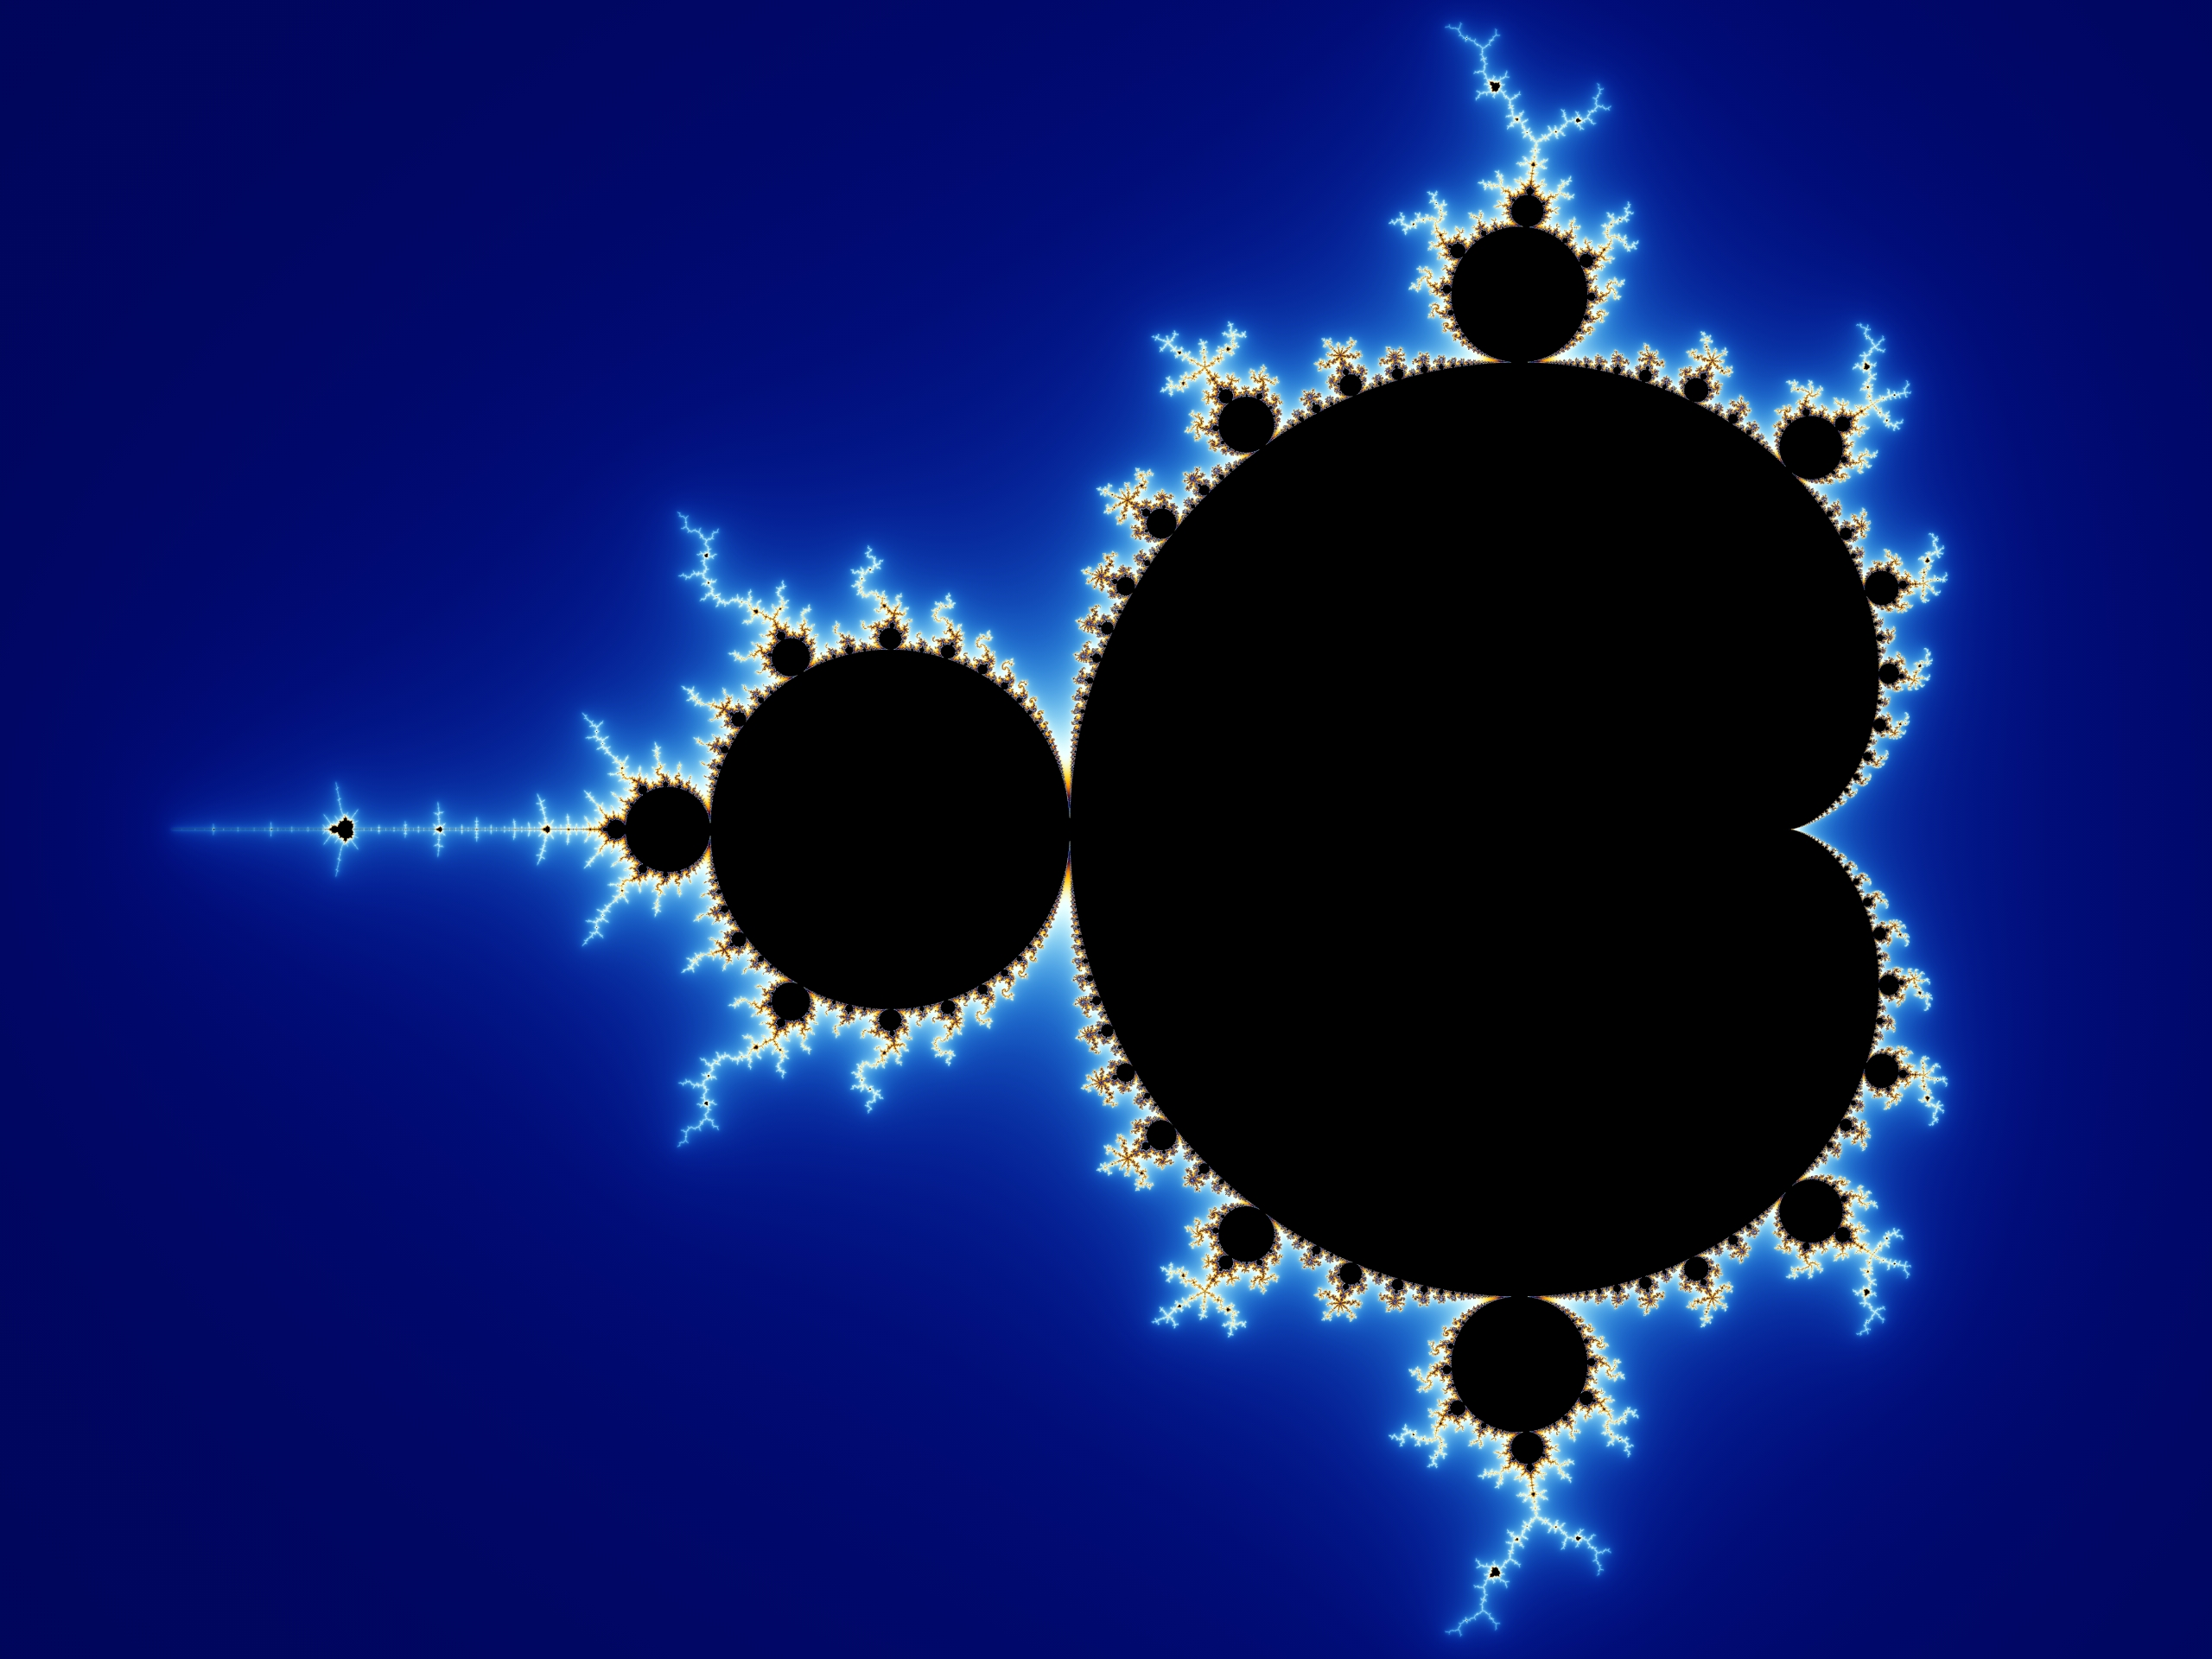
\includegraphics[width=0.8\textwidth]{images/sec-5/mandelbrot}
%     \end{center}
%     \caption[The Mandelbrot fractal]{Image of a Mandelbrot set with a
%         continuously coloured environment. Each pixel corresponds to a point $c$
%         in the complex plane, and its colour depends the number of iterations
%         $n$ before the relation diverges. Centre coordinate
%         $\left( -0.5+0i \right)$, horizontal width 3.2.}
%     \label{fig:mandelbrot}
% \end{figure}
%
% \note{Introduce the (?) operator, talk about what divergence is, why it is bad,
% etc.}
%
% How can we express this computation in a language without iteration? Instead, we
% use generative (meta-programming) techniques to express the recurrence relation.
% Begin by first defining a single step of the relation for a single point in the
% plane. For each point $c$ we keep a pair of elements $\left( z, n \right)$ where
% $z$ is the current value of the relation and $n$ is the iteration that
% divergence occurred at, or the current iteration otherwise.
% %
% \begin{lstlisting}[style=haskell]
% iter :: Exp Complex -> Exp (Complex, Int) -> Exp (Complex, Int)
% iter c z_n = ...
% \end{lstlisting}
% %
% This computes the next value of the polynomial $z_{n+1}$ as well as the number
% of iterations $n$ if the element has not diverged, otherwise returns the value
% and iteration count (at divergence) unchanged. We then lift this to the
% Accelerate array language by applying the operation at all points in the plane
% @cs@:
% %
% \begin{lstlisting}[style=haskell,firstnumber=last]
% step :: Acc (Array DIM2 (Complex,Int)) -> Acc (Array DIM2 (Complex,Int))
% step = A.zipWith iter cs
% \end{lstlisting}
% %
% Note that we have to apply the function even to elements that have already
% diverged. This wastes work but means that there is less SIMD divergence because
% we still do the same thing to every element at every iteration. Here the ``same
% thing'' does imply a small amount if divergence, between elements that have
% already diverged and those that have not, but w
%
% We can then use
% standard Haskell to unroll the loop a \emph{fixed} number of times, which
% completes the Mandelbrot set calculation:
% %
% \begin{lstlisting}[style=haskell,firstnumber=last]
% mandelbrot :: Acc (Array DIM2 (Complex,Int)) -> Acc (Array DIM2 (Complex,Int))
% mandelbrot = foldr ($) zs0 (replicate depth step)
% \end{lstlisting}
% %
% Here @foldr@ and @replicate@ come from the standard Haskell
% prelude, and @depth@ is the maximum iteration count of the relation.
%
% This correctly computes the Mandelbrot set, but is outrageously slow because it
% must read and write the values $z$ and $n$ to memory at each step of the
% computation, rather than keeping these values in registers, computing the entire
% recurrence relation and storing only the final result to memory. Later, we will
% see how the technique of \emph{array fusion} (\S\ref{sec:array_fusion}) can be used to
% eliminate this intermediate memory traffic by combining the \emph{depth}
% applications of the collective operation @zipWith iter@ into a single
% operation containing @depth@ instances of the scalar function
% @iter@, which does not require us to write the intermediate values to
% memory. However, doing this we uncover an embarrassing secret: \emph{a C
% compiler does not compile C code}, it compiles \emph{idiomatic} C code. While
% combining the sequence of collective operations into a single collective
% operation containing a sequence of scalar operations produces faster code due to
% reduced memory traffic, it is still far from optimal.
%
% The problem is that fusing the collective operations in this way does not
% preserve the iteration structure of the recurrence relation, and the loop is
% completely unrolled in the single fused operation. We can introduce scalar loops
% by looking for the following pattern:
% %
% \begin{lstlisting}[style=Haskell,numbers=none,mathescape]
% %\bf$\langle$ loop introduction $\rangle$%
%     let x =
%         let y = e1
%         in e2
%     in e3
%     $\mapsto$
%     iterate[2] (\y -> e2) e1            %\rm if \texttt{e2} $\equiv$ \texttt{e3}%
% \end{lstlisting}
% %
% The nested bindings are replaced with an explicit scalar value iteration
% structure, where the expression @e2@ is repeated twice with the initial
% value @e1@. Similarly, loops can be joined:
% %
% \begin{lstlisting}[style=Haskell,numbers=none,mathescape]
% %\bf$\langle$ loop joining $\rangle$%
%     let x = iterate[n] f e1
%     in e2
%     $\mapsto$
%     iterate[n+1] f e1                   %\rm if the body of \texttt{f} $\equiv$ \texttt{e2}%
% \end{lstlisting}
% %
% Recovering scalar loops in this way enables a backend to generate explicit loops
% in its target language, such as CUDA, and ultimately results in higher
% performance code. In future, it would be beneficial to augment it with related
% loop optimisations such as loop invariant code motion in the frontend and
% lower-level code generation optimisations in a backend.


\section{Related Work}
\label{sec:fusion_related_work}

The desire to program in a functional style while still achieving the
performance level of an imperative language has been around for as long as
functional programming itself. Fusion has received plenty of attention in the
context of functional program. This section briefly summarises some of the
related work in this area.


\subsection{Short-cut fusion}

Most practically successful fusions systems are \emph{short-cut fusion}
\index{fusion!short-cut} methods that rely on local program transformations, and
are implemented as simple but specific rewrite rules combined with general
purpose program transformations. The fusion system employed by Accelerate is in
this vein.

% Inspired by earlier work in @fold/unfold@ methods~\cite{Burstall:1977kl},
% deforestation~\cite{Wadler:1981hy,Wadler:1990ix} applies a set of rewrite rules
% to combinations of common operations such as @map@, @reduce@ and @generate@ in
% order to remove intermediate data structures. While simple, each optimisation
% requires a separate transformation rule for every combination of operators.

@foldr/build@ fusion~\cite{Gill:1996tf,Gill:1993de}\index{fusion!foldr/build}
instead implements library operations out of two basic functions: @build@
constructs a list while @foldr@ consumes it, and a single rewrite rule suffices
to remove intermediate structures. However, not all operations can be expressed
in terms of these two operations, and the transformation does not handle
functions with accumulators (@foldl@) or that consume multiple inputs (@zip@).

Stream fusion~\cite{Coutts:2007kp}\index{fusion!stream} addresses the
shortcomings of @foldr/build@ fusion, while remaining simple and useful in
practice. Operations in the library are written in terms of the @Stream@ data
type, which consists of some abstract state and a stepper function that advances
the stream to the next state. A single rule eliminates matching pairs of
constructor and destructor.


\subsection{Fusion in a parallel context}

Repa~\cite{Keller:2010er} is a Haskell library for parallel array programming on
shared-memory SMP machines. Repa\index{fusion!delayed array} uses a split
representation of arrays as either \emph{delayed} or \emph{manifest}, on which
the @DelayedOpenAcc@ type is based (\S\ref{sec:implementing_array_fusion}).
Representing arrays as functions avoids creating unnecessary intermediate
structures, rather than relying on a subsequent fusion transformation to remove
them. With Repa, the conversion between array representations is done manually
and can cause subexpressions to be recomputed rather than stored and reused. In
some cases this may improve runtime performance, but in general such
unrestrained inlining is the most common cause of performance problems in Repa.
In Accelerate, the conversion is automatic and conservative, so that shared
subexpressions are never recomputed.

Obsidian~\cite{Svensson:2008a} is an EDSL in Haskell for GPGPU programming,
where more details of the GPU hardware are exposed to the programmer. Recent
versions of Obsidian~\cite{Claessen:2012hl} implement Repa-style delayed
\emph{pull arrays}\index{fusion!pull array} as well as \emph{push
arrays}\index{fusion!push array}. Whereas a pull array represents a general
producer, a pull array represents a general consumer. Push arrays allow
intermediate programs to be written in continuation passing style
(CPS)\index{continuation passing style}\index{CPS|see{continuation passing
style}}, and helps to compile and fuse append-like operations.
Baracuda~\cite{Larsen:2011fa} is another Haskell EDSL that produces CUDA kernels
but is intended to be used offline. The paper mentions a fusion system that
appears to be based on pull arrays, but the mechanism is not discussed in
detail.

Delite/LMS~\cite{Rompf:2013er} is a parallelisation framework for DSLs in Scala
that uses library-based multi-pass staging to specify complex optimisations in a
modular manner. Delite supports loop fusion for DSLs targeting GPUs using
rewrite rules on the graph-based intermediate language.

NDP2GPU~\cite{Bergstrom:2012bi} compiles NESL code to CUDA. NDP2GPU performs
@map/map@ fusion, but can not fuse any other operations.
NOVA~\cite{Collins:2013wn} is a high-level lisp-like functional language and
compiler for nested data-parallel array operations. It has a fusion system based
on rewrite rules that combines common patterns such as @map/map@ and @map/fold@.

\citet{Sato:2009cq} describe a C++ skeleton-based library for GPGPU programming
that additionally includes a source-to-source fusion mechanism based on list
homomorphisms. SkeTo~\cite{Matsuzaki:2011ew} is a C++ library that provides
parallel skeletons for CPUs. SkeTo's use of C++ templates provides a fusion
system similar to delayed arrays, which would be equivalently implemented using
CUDA templates.


tk: dandelion~\cite{Rossbach:2013bj}, series
expressions/repa-4~\cite{Lippmeier:2013vz}, hylomorphism
fusion~\cite{Takano:1995}, loop fusion from imperative
languages~\cite{Warren:1984ka,Sarkar:1991ff}.


% \subsection{Deforestation}
%
% % blugh blurgh
% Inspired by earlier work in @fold/unfold@ methods (for example
% \citet{Burstall:1977kl}), Philip Wadler set out to develop a technique that
% would \emph{automatically} remove intermediate structures from functional
% programs, a technique he (later) dubbed \indexe{deforestation}
% \cite{Wadler:1981hy,Wadler:1990ix}.
%
% The method identifies a core set of list operators that can be used to express a
% large class of computations: @map@, @reduce@ and @generate@ (the
% latter being similar in spirit to @foldr@ and @unfoldr@ respectively),
% together with a collection of rewrite rules that apply to combinations of these
% operators. These rules identify specific patterns of list operators that create
% then consume intermediate lists, then merges these operations to avoid the
% intermediary.
%
% \paragraph{Advantages}
% \begin{itemize}
%     \item Automatic: does not require programmer input, and therefore suitable
%         for integration to a compiler.
%
%     \item Source-to-source: all transformations take valid programs in the
%         source language and output (faster) valid programs in the source
%         language. This makes the output of deforestation easy to integrate as
%         part of a compiler pipeline.
%
%     \item Simple: each rule is easy to understand and obviously correct.
% \end{itemize}
%
% \paragraph{Disadvantages}
% \begin{itemize}
%     \item Each optimisation requires a separate transformation rule. If we want
%         to add new list operators, we need to add a new rule for each
%         combination of the new operator with each existing operator. This does
%         not scale.
%
%     \item Limited: many computations can not be expressed in terms of these
%         three operations, so the framework can not eliminate intermediate lists
%         in these case.
% \end{itemize}
%
%
% \subsection{foldr/build}
%
% Building upon the original deforestation algorithm, Andy Gill's doctoral thesis
% introduces another approach to deforestation known as \emph{foldr/build
% fusion}~\cite{Gill:1996tf,Gill:1993de}.
% \index{fusion!foldr/build}\index{foldr/build|see{fusion!foldr/build}}
% % This techniques performs a range of optimisations as broad as previous
% % approaches the listless transformer \cite{Wadler:1984ia,Wadler:2005iw} while
% % addressing their drawbacks.
% Like the deforestation algorithm, @foldr/build@ fusion is a rule-based
% source-to-source transformation. In fact, it is based on a single rule:
% %
% \begin{lstlisting}[style=Haskell
%     ,numbers=none
%     ,mathescape
%     ,caption={The \code{foldr/build} transformation}]
% %\bf$\langle$ foldr/build fusion $\rangle$% forall g k z. foldr k z (build g) $\mapsto$ g k z
%
% build :: (forall b. (a -> b -> b) -> b -> b) -> [a]
% foldr :: (a -> b -> b) -> b -> [a] -> b
% \end{lstlisting}
%
% The idea is to think of @build@ as a function that constructs a list, and
% @foldr@ as a list consumer. Because of this uniform treatment of lists as
% \emph{complete objects}, rather than being composed of many individual
% constructor cells, we can have a single @foldr/build@ rule analogous to
% standard case reduction rules, but instead of removing a single constructor
% removes the \emph{entire data structure}. This method became the first
% non-trivial deforestation system to be included as an active part of a
% production quality functional language compiler.
%
% \paragraph{Advantages}
% \begin{itemize}
%     \item Simple, automatic, source-to-source transformation.
%
% %    \item No limitation on inputs: @foldr/build@ fusion operates over the
% %        entire Haskell language. When a list is produced without using
% %        @build@ or consumed without using @foldr@, the
% %        deforestation scheme is not hampered and simply leaves the list intact.
%
%     \item Single rule: unlike the original deforestation algorithm, a single
%         rule suffices. When new list operations are added, so long as they can
%         be expressed in terms of @foldr@ and @build@, the
%         transformation will apply; there is no need to consider all combinations
%         with the existing operations.
% \end{itemize}
%
% \paragraph{Disadvantages}
% \begin{itemize}
%     \item The transformation can not handle functions that use accumulators,
%         such as @foldl@, or consume multiple inputs, such as @zip@.
%
%     \item Operations that do not produce lists using @build@ or consume them
%         using @foldr@ will not have the intermediate list eliminated.
% \end{itemize}
%
% \subsection{Stream Fusion}
%
% Following Gill's work, a whole cottage industry of new deforestation approaches
% appeared with the goal of covering the cases left out by
% @foldr/build@\index{fusion!foldr/build}. Most of that work was
% theoretical, a lot of it was based on category theory, and almost none of it had
% any impact in practice. Unlike those systems of the prior two decades,
% \emph{stream fusion}\index{fusion!stream}~\cite{Coutts:2007kp} succeeded in this
% goal and at the same time stayed simple and useful in practice.
%
% As shown in Listing~\ref{lst:stream_fusion}, stream fusion has a similar
% structure to @foldr/build@: a single rule eliminates matching pairs of
% constructor and destructor, and operations need to be expressed in terms of
% these constructors.
% %
% \begin{lstlisting}[style=Haskell
%     ,numbers=none
%     ,mathescape
%     ,float
%     ,label=lst:stream_fusion
%     ,caption={The stream fusion transformation}]
% %\bf$\langle$ stream fusion $\rangle$% forall s. stream (unstream s) $\mapsto$ s
%
% stream   :: [a] -> Stream a
% unstream :: Stream a -> [a]
%
% data Stream a = exists s. Stream (s -> Step a s) s
% data Step a s = Done
%               | Yield a s           -- produce a value and new state
%               | Skip s              -- update the state without producing a value
% \end{lstlisting}
%
% Streams have some abstract state and a \emph{stepper} function that advances the
% stream from one state to the next, possibly yielding a new value. The
% @stream@ constructor @Yield@s values from its input until it runs
% out, and the @unstream@ destructor build a list by consuming its input
% stream until encountering @Done@, discarding @Skip@s along the
% way. The @Stream@ constructors are chosen so as to keep the definition of
% each element as a non-recursive function. When @Stream@s are fused by
% applying the rule, this enables the compiler to aggressively apply standard
% optimisation techniques.
%
% \paragraph{Advantages}
% \begin{itemize}
%     \item Preserves the nice properties of
%         @foldr/build@\index{fusion!foldr/build} fusion.
%     \item Adds supports operations with accumulators and multiple inputs.
% \end{itemize}
%
% \paragraph{Disadvantages}
% \begin{itemize}
%     \item Fuses a sequence of bulk operations into a single scalar loop, losing
%         the parallel interpretation of the program.
% \end{itemize}
%
% \subsection{Data Parallel Haskell}
% tk: @split/join@\index{fusion!split/join} fusion from
% DPH\@.\index{data-parallel Haskell}\index{DPH|see{data-parallel Haskell}}
% \citet{Chakravarty:2007tc,Jones:2008uu}.
%
%
% \subsection{Delayed Arrays}
%
% The previous fusion transformations are based on the idea of expressing
% computations in terms of a builder and consumer function, and then having the
% compiler identify and remove adjacent constructor/destructor pairs. In contrast,
% the Repa~\cite{Keller:2010er} library uses a functional representation of
% \emph{delayed arrays}\index{fusion!delayed arrays} that instead \emph{avoids}
% creating unnecessary intermediate structures, rather than relying on a
% subsequent fusion transformation to remove them. The basic definition of delayed
% arrays --- without the use of indexed types~\cite{Chakravarty:2005kg} to specify
% the representation and computation method~\cite{Lippmeier:2012gx} --- is shown
% in Listing~\ref{lst:repa_arrays}.
%
% \begin{lstlisting}[style=Haskell
%     ,numbers=none
%     ,float
%     ,label={lst:repa_arrays}
%     ,caption={Repa-1 style array definition}]
% data Array sh e = Manifest sh (Vector e)    -- unboxed data
%                 | Delayed  sh (sh -> e)     -- array shape and indexing function
% \end{lstlisting}
%
% The key principle of the design is to avoid generating an explicit
% (@Manifest@) representation of intermediate arrays that can instead be
% represented as a transformation function from array indices to values.
%
% % Repa retains the functional programming style by exposing an interface of
% % collective operations over arrays --- such as maps, folds, and permutations ---
% % instead of the imperative style of reading and writing individual array
% % elements.
%
% \paragraph{Advantages}
% \begin{itemize}
%     \item Explicitly avoids intermediate structures by design, rather than
%         relying on potentially fragile post-hoc compiler transformations.
% \end{itemize}
%
% \paragraph{Disadvantages}
% \begin{itemize}
%     \item Requires the user to explicitly state when arrays should be computed
%         (made manifest), else performance suffers due to redundant computation.
% \end{itemize}
%
% \subsection{Hylomorphism fusion}
% tk: \citet{Takano:1995}
%
% \subsection{Loop fusion}
% From imperative languages. tk: \citet{Warren:1984ka,Sarkar:1991ff}
%
%
% \subsection{Conclusion}
%
% The most practically successful fusion systems ---
% @foldr/build@\index{fusion!foldr/build} fusion, stream\index{fusion!stream}
% fusion and delayed arrays\index{fusion!delayed arrays} --- are \emph{short-cut
% fusion}\index{fusion!short-cut} methods that rely on local program
% transformations. These methods are implemented as simple but specific rewrite
% rules combined with general purpose program transformations.
%
% In contrast, \emph{loop fusion}\index{fusion!loop} methods used in imperative
% languages merge multiple loop nests, typically using dependency
% graphs to determine whether fusion is legal and beneficial.
% When a producer and consumer loop are merged, array
% contraction can then remove or reduce the size of the
% intermediate arrays. These systems require fusion-specific compiler support and
% more global reasoning than short-cut fusion.


\section{Discussion}

This chapter has detailed our approach to optimising programs written in
Accelerate, a language of parallel array operations suitable execution on
bulk-parallel SIMD architectures such as GPUs and multicore CPUs. Our previous
work identified sharing and array fusion as the key bottlenecks to achieving
high performance. This chapter discusses our novel approaches that tackle these
problems. While we motivate our approaches in the context of Accelerate, both
approaches are more widely applicable. In particular, our sharing recovery
algorithm applies to any embedded language based on the typed lambda calculus,
and our array fusion optimisation applies to any dynamic compiler targeting
SIMD hardware.

The set of optimisations that have been described in this chapter can be seen as
a set of term rewriting rules. We would like this set of transformations to be:
%
\begin{itemize}
    \item \emph{Correct:} The transformed code retains the same semantics as the
        original code.

    \item \emph{Improving efficiency:} The transformed code should require less
        time and/or fewer resources to execute than the original. We address
        this through a series of benchmarks in chapter~\ref{ch:results}.
\end{itemize}
%
In addition, it would be of significant practical advantage if the
transformations were:
%
\begin{itemize}
    \item \emph{Confluent:} When more than one transformation is applicable to a
        given term, applying the transformations in any ordering should yield
        the same result. This is important to ensure that opportunities to apply
        transformations are not lost, or worse code is generated, due to the
        choice of applying one transformation before another.

    \item \emph{Terminating:} We reach a point when no transformation is
        applicable so the simplification process stops. One must be careful that
        one transformation [sequence] can not generate terms that can be
        transformed back to the original; that no transformation undoes the work
        of another.
\end{itemize}


\subsection{Correctness}

Fusion systems such as \texttt{foldr/build}~\cite{Gill:1993de} and the system
presented here, work by eliminating intermediate data structures. Since these
transformations are performed automatically by the compiler, we would like to be
sure that the left and right hand side of the rewrite are equivalences.
In particular, we are concerned as to whether:
%
\begin{enumerate}
    \item Can a safely terminating program be transformed into a failing one?
    \item Can a safely terminating program be transformed into another safely
        terminating program that gives a different value as the result?
\end{enumerate}

For \texttt{foldr/build} fusion applied to regular Haskell lists, it is possible
to distinguish cases where the two sides of the transformation are not
equivalent. Breaking semantic equivalence for \texttt{foldr/build} requires the
use of the special operator @seq@, which evaluates its first argument to head
normal form.%
\footnote{Recall that Haskell has non-strict evaluation semantics. This means,
for example, that it is possibly to evaluate the length of the following list,
even though the second list element raises an error, because the individual list
elements are never demanded: \footcode{length [1, error "boom!", 3]} $\mapsto$
\footcode{3}. However, if we were to first apply \footcode{seq} to each list
element in order to demand its evaluation, then the error will be raised, and
our program will fail.}
We avoid this issue because the Accelerate language itself is strict: every term
in the language always evaluates to a value. An operator like @seq@ to force
evaluation is thus unnecessary, and can not be used to distinguish fused and
unfused programs.

The Accelerate language does not have an explicit term to represent exceptional
values. However, it is possible to compute undefined values, such as division by
zero. Consider the following program:
%
\begin{lstlisting}[style=haskell]
xs :: Acc (Vector Float)
xs = map (\x -> 131.95 / x)                                             -- [42, $\infty$, $\infty$, \ldots]
   $ generate (constant (Z:.10))                                        -- [3.14159, 0, 0, \ldots]
              (\ix -> let i = unindex1 ix in i ==* 0 ? (%$\pi$%, 0))
\end{lstlisting}
%
Evaluating this program, the second and subsequent entries in the array evaluate
to infinity, as the program attempts to divide by zero. However, if we were to
use this term in the following program that extracts only the first value:
%
\begin{lstlisting}[style=haskell]
unit (xs ! constant (Z:.0)) %$\mapsto$% unit 42
\end{lstlisting}
%
The program is fused into a single operation that no longer performs the
division by zero. If we classify invalid arithmetic as a kind of program
failure, then the fusion system presented in this chapter has just transformed a
failing program into a safely terminating program, because the intermediate
states that performed the invalid operations have been eliminated. It is left to
future work to provide a formal proof that the converse can not happen.


\subsection{Confluence and termination}

The array fusion transformation (\S\ref{sec:implementing_array_fusion}) is
designed to be a single-pass algorithm that specifies only a single rewrite to
be applied at each node. Thus, the transformation does not need to select from a
set of possible rewrites to apply or the order in which to apply them, based on
heuristics or otherwise. Since the delayed representation of producers is
non-recursive (Listing~\ref{lst:cunctation}), referencing input arrays via
environment indices rather than as general terms, a subsequent shrinking pass
(\S\ref{sec:shrinking}) is not required to eliminate or combine the uses of
bound variables. Hence, it is not necessary to iterate the fusion and shrinking
steps, so that shrinking can expose all opportunities for fusion.

Informally, then, we are confident that the fusion transformation is both
confluent and terminating. Furthermore, since we fuse programs by rewriting
typed de Bruijn terms in a type preserving manner, we are confident that each
individual rewrite is correct, since the type information amounts to a partial
proof of correctness checked by the type checker.


\subsection{Error tests eliminated}

Collective operations in Accelerate are rank polymorphic. For example, @fold@
reduces along the innermost dimension of an array, reducing the rank of that
array by one. The @reshape@ operation allows us to change the shape of an array
without altering its contents. This is useful to, for example, reduce an array
of arbitrary rank to a single value:
%
\begin{lstlisting}[style=haskell]
foldAll :: (Shape sh, Elt e)
        => (Exp e -> Exp e -> Exp e)
        -> Exp e
        -> Acc (Array sh e)
        -> Acc (Scalar e)
foldAll f z a = fold f z $ reshape (index1 (size a)) a
\end{lstlisting}
%
In order to reshape arrays efficiently, we require that the size of the source
and result arrays are identical. This allows the runtime to simply change the
interpretation of the array, without touching the actual data, and is thus a
constant-time operation. This precondition must be checked at runtime, and an
error generated if the sizes do not match.

However, the @reshape@ operation is also a general producer
(Listing~\ref{lst:producer_consumer_operations}), and can thus be fused into
other operations. If this happens, the runtime can no longer check the
precondition on the host --- because the term has been removed from the source
program --- and since it is not possible to throw exceptions from massively
parallel GPU code, fusion has effectively eliminated the runtime error check.

It is left for future work to add the ability to represent error terms in the
embedded language. For @reshape@ --- currently the only term which includes a
runtime test --- we minimise the loss of the error test by only fusing the
operation into delayed terms, while still emitting the @reshape@ term whenever
it is applied to manifest data, in order to preserve the error test for this
case.


\subsection{Work duplication}

While the fusion transformation is cautious and only fuses producer terms that
have a single use site, it is still possible to introduce some amount of work
duplication. For example, fusing an operation such as @replicate sh (map f xs)@
results in the function @f@ being applied a number of times equal to the size of
the resulting shape @sh@, rather than the size of the source array @xs@. If @f@
is expensive or @sh@ is large, even though there is a single use site for the
source array @xs@, it might still be beneficial to not fuse these terms.

The second source of work duplication can arise through the use of array
indexing. At an example, consider the following function, where each element of
the array @xs@ is repeated four times sequentially in the result, i.e.
@[a,b,c]@ $\mapsto$ @[a,a,a,a,b,b,b,b,c,c,c,c]@:
%
\begin{lstlisting}[style=haskell]
quad = generate sh (\ix -> xs ! ilift1 (`div` 4) ix)
  where
    sh = index1 (size xs * 4)
    xs = map f (use (Array ...))
\end{lstlisting}
%
Since @xs@ has a single use site in @generate@, the function @f@ will be fused
directly into this location. The fusion transformation has thus just committed
to evaluating @f@ four times more than was specified in the original program.

For GPUs, which support thousands of active threads, recomputing values to
reduce memory bandwidth is usually beneficial, but for a CPU with relatively few
cores, this might not be the case. Allowing users to explicitly specify in the
source language which terms should always be computed to memory, or conversely
fused unconditionally, is left to future work. Adding an analysis that estimates
when such work duplication is beneficial is also left to future work.


\subsection{Ordering and repeated evaluations}

There are several possible orderings for the transformation passes that have
been discussed in this chapter, and it would be possible to invent examples to
show that no one order can be optimal for all programs.

As described above, the array fusion pass is designed so that it only needs to
be applied to the source program once, and not iterated with the shrinking step
in order to expose all opportunities for fusion. However, for the case of
let-elimination, if the bound term is eliminated by inlining it directly into
the body, then the new redex must be re-traversed. For the fusion
transformation, let-elimination is the only reason a term might be inspected
more than once.

On the other hand, scalar expressions must alternate between the simplification
and shrinking steps. Thus, we must decide in which order to apply the two
operations. Because the shrinking step changes the structure of the AST by
removing let bindings, which might be useful for the simplification analysis,%
\footnote{In particular, before the introduction of an explicit value recursion
term into the source language, uses encoded iteration by defining a single step
of the loop body as a collective operation, and using Haskell to repeatedly
apply it, effectively unrolling the loop a fixed number of times. Fusion would
then combine these $n$ collective operations into a single operation containing
$n$ instances of the loop body. However, it was found that the CUDA compiler was
not well suited to compiling the manually unrolled loop C compilers don't
compile C code, they compile \emph{idiomatic} C code. The loop recovery
simplification was thus designed to convert the unrolled loop body back into an
explicit iteration form, and in part this relied on the structure of let terms,
which could be obfuscated by shrinking. Following the introduction of explicit
iteration, loop recovery has since been disabled.}
we perform scalar simplifications before shrinking. Moreover, both the
simplification and shrinking operations return a boolean indicating whether or
not the operation made any changes to the AST. The scalar optimisation pipeline
applies one round of simplification, then iterates shrinking and simplification
until the expression no longer changes, or the limit of two applications of each
operation is reached.


% \section*{NOTES}
%
% MMTC: Chapter 5: This set up where you put the related work for fusion in the
% middle of the chapter doesn't work IMO\@. Always lead with the interesting
% material (your contribution) and not with the boring stuff (previous work that
% expert readers already know anyway). Put the related work at the end of the
% chapter.
%
% Section 5.3 (typed equality) seems out of place. (You have got a remark to maybe
% move it to implementation. I'm not sure whether that is the right place, but the
% current place is definitely not good.)
%
% Section 5.4 \& 5.5 (simultaneous substitution and environment manipulation) also
% seem like a distraction in the middle of explaining fusion. First you have the
% general fusion setup in 5.2 and then the details in 5.6. They should one
% straight after the other without any distraction in between. If you need 5.4 \&
% 5.5 for 5.6, then make sure you discuss this stuff earlier. Maybe it should be
% part of the background or the implementation chapter.
%
% MMTC: Section numbers with 4 parts (5.2.2.1 etc) look silly. Use unnumbered
% paragraph's or revise your structure.

